\documentclass[a4paper]{book}
\usepackage{makeidx}
\usepackage{graphicx}
\usepackage{multicol}
\usepackage{float}
\usepackage{listings}
\usepackage{color}
\usepackage{ifthen}
\usepackage[table]{xcolor}
\usepackage{textcomp}
\usepackage{alltt}
\usepackage{ifpdf}
\ifpdf
\usepackage[pdftex,
            pagebackref=true,
            colorlinks=true,
            linkcolor=blue,
            unicode
           ]{hyperref}
\else
\usepackage[ps2pdf,
            pagebackref=true,
            colorlinks=true,
            linkcolor=blue,
            unicode
           ]{hyperref}
\usepackage{pspicture}
\fi
\usepackage[utf8]{inputenc}
\usepackage[ngerman]{babel}

\usepackage{mathptmx}
\usepackage[scaled=.90]{helvet}
\usepackage{courier}
\usepackage{sectsty}
\usepackage[titles]{tocloft}
\usepackage{doxygen}
\lstset{language=C++,inputencoding=utf8,basicstyle=\footnotesize,breaklines=true,breakatwhitespace=true,tabsize=3,numbers=left }
\makeindex
\setcounter{tocdepth}{3}
\renewcommand{\footrulewidth}{0.4pt}
\renewcommand{\familydefault}{\sfdefault}
\begin{document}
\hypersetup{pageanchor=false}
\begin{titlepage}
\vspace*{7cm}
\begin{center}
{\Large ardrone\_\-swp }\\
\vspace*{1cm}
{\large Erzeugt von Doxygen 1.7.4}\\
\vspace*{0.5cm}
{\small Tue Sep 4 2012 16:08:00}\\
\end{center}
\end{titlepage}
\clearemptydoublepage
\pagenumbering{roman}
\tableofcontents
\clearemptydoublepage
\pagenumbering{arabic}
\hypersetup{pageanchor=true}
\chapter{Hauptseite}
\label{index}\hypertarget{index}{}

\subsection*{Was machen die Apps? }

\subsubsection*{\hyperlink{bottom__follow__tag_8cpp}{bottom\_\-follow\_\-tag.cpp} }

Diese Applikation wurde dazu entwickelt, dass die Drone einem Tag, welches auf einem Bodenroboter befestigt wurde, zu folgen. Dabei muss die Drone extern mittels Dronenbefehl gestartet werden und dann zum Bodenroboter bewegt werden, damit sie das Tag erfassen kann. Ab diesem Augenblick wird die Drone versuchen immer über dem Tag zu stehen und sich ausrichten. Der Bodenroboter kann sich von nun an bewegen und wird über sich von der Drone verfolgt.

\subsubsection*{\hyperlink{front__follow__tag_8cpp}{front\_\-follow\_\-tag.cpp} }

Diese Applikation dient dazu, dass die Drone einem Tag oder Marker folgt welches sie an ihrer vorderen Kamera sieht. Dabei versucht die Drone ca. einen Meter vor dem Tag zu stehen und senkrecht auf das Tag zu schauen. Sobald die Drone das Tag einmal erkannt hat, wird sie von nun an versuchen ihre Position gegenüber dem Tag zu halten, was einem Folgen gleichkommt. Dabei wird die Drone sich in alle Richtungen frei bewegen, außer in der Höhe haben wir eine Tiefst-\/ und Höchstbegrenzung implementiert.

Im Ordner Bilder sind die Marker zu finden.

\subsubsection*{\hyperlink{follow__line_8cpp}{follow\_\-line.cpp} }

Diese Applikation wurde dazu entwickelt, dass die Drone einer schwarzen Linie auf hellem Untergrund folgt. Der Kontrast sollte möglichst hoch sein. Dabei ist zu beachten, dass die Kurven der Linie möglichst aus Ecken und Geraden besteht. Also extrapoliert würde ein zu fliegender Kreis wie ein Polygon mit mindestens 10 Ecken sein.



Dieses Bild verdeutlicht den Zusammenhang zwischen unseren Applikationen und der von uns verwendeten externen Software.

\subsection*{Installation von ROS, dem Brown-\/Pkg und den Applikationen. }

Für unsere drei Applikationen verwendeten wir ROS(Robotic Operation System) und den Ardrone Treiber der Brown Universität. Für die richtige Installation und Anwendung der Applikationen ist dieser Guide da. Da wird den Browntreiber verändert haben, sollte unbedingt unsere Version des Treibers verwendet werden.

Die Apps wurden auf Ubuntu 11.10. und mit der ROS Version Electric erstellt und da den Apps kein Support untersteht, kann es mit neueren Versionen gegebenenfalls zu Problemen kommen. Eine aktuelle Installationsanleitung finden sie unter dem folgenden Link: \href{http://www.ros.org/wiki/ROS/Installation}{\tt http://www.ros.org/wiki/ROS/Installation}

\subparagraph*{Ros }

$>$ sudo sh -\/c 'echo \char`\"{}deb http://packages.ros.org/ros/ubuntu electric main\char`\"{} $>$ /etc/apt/sources.list.d/ros-\/latest.list'

$>$ wget \href{http://packages.ros.org/ros.key}{\tt http://packages.ros.org/ros.key} -\/O -\/ $|$ sudo apt-\/key add -\/

$>$ sudo apt-\/get update

$>$ sudo apt-\/get install ros-\/electric-\/desktop

$>$ echo \char`\"{}source /opt/ros/electric/setup.bash\char`\"{} $>$$>$ $\sim$/.bashrc

$>$ . $\sim$/.bashrc

\subparagraph*{Brown-\/Pkg }

$>$ sudo apt-\/get install ros-\/electric-\/brown-\/drivers

$>$ sudo apt-\/get install ros-\/electric-\/brown-\/remotelab

$>$ sudo apt-\/get install ros-\/electric-\/joystick-\/drivers

$>$ sudo apt-\/get install guvcview

$>$ sudo apt-\/get install libsdl1.2-\/dev

$>$ cd $\sim$

$>$ mkdir ros

$>$ cd ros

$>$ svn checkout \href{https://svn-eos.cs.ovgu.de/repos/stud/riestock}{\tt https://svn-\/eos.cs.ovgu.de/repos/stud/riestock}

$>$ export ROS\_\-PACKAGE\_\-PATH=/home/maik/ros:\$ROS\_\-PACKAGE\_\-PATH

Bei der Pfadangabe bitte darauf achten euren Anmeldenamen zu verwenden.

$>$ cd /home/maik/ros/brown-\/ros-\/pkg/experimental/ardrone\_\-brown

$>$ ./build\_\-sdk.sh

$>$ cmake .

$>$ rosmake ardrone\_\-brown

\subparagraph*{Recog }

$>$ cd /home/maik/ros/brown-\/ros-\/pkg/experimental/ar\_\-recog

$>$ cmake .

$>$ rosmake ar\_\-recog

\subparagraph*{Applikationen }

$>$ rosmake ardrone\_\-swp

\subsection*{Wie startet man die Apps? }

Um die Apps zu verwenden brauch man eine Menge von Terminals. Wir haben die Arten der Befehle in 4 Bereiche untergliedert. Als Erstes die Befehle die nötig sind um den Roskern zu starten, welches immer am Anfang geschehen muss. Danach die Befehlsequenze für die drei Apps. Am Ende sind noch einmal die Terminalbefehle, welche direkt die Drone steuern, und zusätzliche Befehle.

\subsubsection*{Roskern und Brown-\/Treiber }

$>$ rosrun roscore

$>$ rosrun ardrone\_\-brown ardrone\_\-driver

\subsubsection*{Applikationen }

\subparagraph*{bottom\_\-follow\_\-tag }

$>$ rosservice call /ardrone/togglecam

$>$ roscd ar\_\-recog/bin

$>$ rosparam set aov 0.001

$>$ rosrun ar\_\-recog ar\_\-recog image:=/ardrone/image\_\-raw

$>$ rostopic pub /ardrone/takeoff std\_\-msgs/Empty

$>$ rosrun ardrone\_\-swp bottom\_\-follow\_\-tag

am Ende zum Landen $>$ rostopic pub /ardrone/land std\_\-msgs/Empty

\subparagraph*{front\_\-follow\_\-tag }

$>$ roscd ar\_\-recog/bin

$>$ rosparam set aov 0.001

$>$ rosrun ar\_\-recog ar\_\-recog image:=/ardrone/image\_\-raw

$>$ rostopic pub /ardrone/takeoff std\_\-msgs/Empty

$>$ rosrun ardrone\_\-swp front\_\-follow\_\-tag

am Ende zum Landen $>$ rostopic pub /ardrone/land std\_\-msgs/Empty

\subparagraph*{follow\_\-line }

$>$ rosservice call /ardrone/togglecam

$>$ rosrun ardrone\_\-swp \hyperlink{_track_line_8py}{TrackLine.py}

$>$ rostopic pub /ardrone/takeoff std\_\-msgs/Empty

$>$ rosrun ardrone\_\-swp follow\_\-line

am Ende zum Landen $>$ rostopic pub /ardrone/land std\_\-msgs/Empty

\subsubsection*{Steuerung }

$>$ rostopic pub /ardrone/takeoff std\_\-msgs/Empty Mit diesem Kommando wird die Drone jedes mal gestartet.

$>$ rostopic pub /ardrone/land std\_\-msgs/Empty Mit diesem Kommando wird die Drone jedes mal gelandet.

$>$ rostopic pub /ardrone/reset std\_\-msgs/Empty Mit diesem Kommando kann die Drone resetet werden, falls die Drone in den Notfallmodus geht.

\subsubsection*{zusätzliche Befehle }

Durch diesen Befehl wird das aktuelle Kamerabild ausgegeben: $>$ rosrun image\_\-view image\_\-view image:=/ardrone/image\_\-raw

Durch diese Befehle werden die reinkommenden Nachrichten des Typs /tags bzw. /ardrone/navdata auf die Konsole geschrieben:

$>$ rostopic echo /tags

$>$ rostopic echo /ardrone/navdata

Durch das folgende Kommando wird ein zusätzliches Programm gestartet, welche die Navigationsdaten, Tagdaten und/oder die Steuerungsbefehle aufzeichnet:

$>$ ardrone\_\-swp Log $<$options$>$ -\/$>$ $<$n$>$ für die navdata, $<$t$>$ für die Informationen der Tags, $<$w$>$ für die gesendeten Steuerungsbefehle

Als Beispiel:

$>$ ardrone\_\-swp Log n w Jetzt protokolliert das Programm alle grad erzeugten navdata und gesendeten Steuerungsbefehle und speichert diese in ardrone\_\-swp/Log. 
\chapter{Verzeichnishierarchie}
\section{Verzeichnisse}
Diese Verzeichnishierarchie ist -\/mit Einschränkungen-\/ alphabetisch sortiert:\begin{DoxyCompactList}
\item \contentsline{section}{include}{\pageref{dir_39166a97d2c880e9e8380b0ac096fb0d}}{}
\item \contentsline{section}{src}{\pageref{dir_8825dd29552366a97c79ae3282986fe7}}{}
\end{DoxyCompactList}

\chapter{Verzeichnis der Namensbereiche}
\section{Liste aller Namensbereiche}
Liste aller Namensbereiche mit Kurzbeschreibung:\begin{DoxyCompactList}
\item\contentsline{section}{\hyperlink{namespaceanonymous__namespace_02_math_8cpp_03}{anonymous\_\-namespace\{Math.cpp\}} }{\pageref{namespaceanonymous__namespace_02_math_8cpp_03}}{}
\item\contentsline{section}{\hyperlink{namespace_keyboard}{Keyboard} (Enthält \hyperlink{namespace_keyboard_abfb3168172d115a6516147c6d42f58db}{Keyboard::control()} zum steuern der Drone mit der Tastatur )}{\pageref{namespace_keyboard}}{}
\item\contentsline{section}{\hyperlink{namespace_math}{Math} (Enthält Funktionen für das Berechen wo sich ein Tag bezüglich des Bildes befindet und die Regelung )}{\pageref{namespace_math}}{}
\item\contentsline{section}{\hyperlink{namespace_track_line}{TrackLine} }{\pageref{namespace_track_line}}{}
\end{DoxyCompactList}

\chapter{Klassen-\/Verzeichnis}
\section{Auflistung der Klassen}
Hier folgt die Aufzählung aller Klassen, Strukturen, Varianten und Schnittstellen mit einer Kurzbeschreibung:\begin{DoxyCompactList}
\item\contentsline{section}{\hyperlink{class_cglobal}{Cglobal} }{\pageref{class_cglobal}}{}
\item\contentsline{section}{\hyperlink{class_delta}{Delta} }{\pageref{class_delta}}{}
\end{DoxyCompactList}

\chapter{Datei-\/Verzeichnis}
\section{Auflistung der Dateien}
Hier folgt die Aufzählung aller Dateien mit einer Kurzbeschreibung:\begin{DoxyCompactList}
\item\contentsline{section}{include/\hyperlink{_delta_8h}{Delta.h} }{\pageref{_delta_8h}}{}
\item\contentsline{section}{include/\hyperlink{_global_8h}{Global.h} }{\pageref{_global_8h}}{}
\item\contentsline{section}{include/\hyperlink{_keyboard_8h}{Keyboard.h} }{\pageref{_keyboard_8h}}{}
\item\contentsline{section}{include/\hyperlink{_math_8h}{Math.h} }{\pageref{_math_8h}}{}
\item\contentsline{section}{include/\hyperlink{std__includes_8h}{std\_\-includes.h} }{\pageref{std__includes_8h}}{}
\item\contentsline{section}{src/\hyperlink{bottom__follow__tag_8cpp}{bottom\_\-follow\_\-tag.cpp} (Applikation zur Tagvervolgung mit der unteren Kamera )}{\pageref{bottom__follow__tag_8cpp}}{}
\item\contentsline{section}{src/\hyperlink{_delta_8cpp}{Delta.cpp} }{\pageref{_delta_8cpp}}{}
\item\contentsline{section}{src/\hyperlink{follow__line_8cpp}{follow\_\-line.cpp} (Applikation zur Linienverfolgung mit der unteren Kamera )}{\pageref{follow__line_8cpp}}{}
\item\contentsline{section}{src/\hyperlink{front__follow__tag_8cpp}{front\_\-follow\_\-tag.cpp} (Applikation zur Tagvervolgung mit der vorderen Kamera )}{\pageref{front__follow__tag_8cpp}}{}
\item\contentsline{section}{src/\hyperlink{_global_8cpp}{Global.cpp} }{\pageref{_global_8cpp}}{}
\item\contentsline{section}{src/\hyperlink{_keyboard_8cpp}{Keyboard.cpp} }{\pageref{_keyboard_8cpp}}{}
\item\contentsline{section}{src/\hyperlink{_log_8cpp}{Log.cpp} }{\pageref{_log_8cpp}}{}
\item\contentsline{section}{src/\hyperlink{_math_8cpp}{Math.cpp} }{\pageref{_math_8cpp}}{}
\end{DoxyCompactList}

\chapter{Verzeichnisdokumentation}
\hypertarget{dir_39166a97d2c880e9e8380b0ac096fb0d}{
\section{include/-\/Verzeichnisreferenz}
\label{dir_39166a97d2c880e9e8380b0ac096fb0d}\index{include/-\/Verzeichnisreferenz@{include/-\/Verzeichnisreferenz}}
}
Directory dependency graph for include/:\nopagebreak
\begin{figure}[H]
\begin{center}
\leavevmode
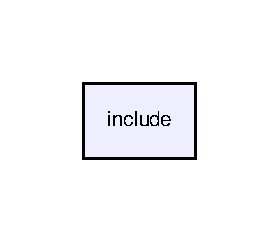
\includegraphics[width=134pt]{dir_39166a97d2c880e9e8380b0ac096fb0d_dep}
\end{center}
\end{figure}
\subsection*{Dateien}
\begin{DoxyCompactItemize}
\item 
Datei \hyperlink{_delta_8h}{Delta.h}


\begin{DoxyCompactList}\small\item\em Klasse, zur Berechnung der Geschwindigkeit (wird nicht mehr verwendet) \end{DoxyCompactList}

\item 
Datei \hyperlink{_global_8h}{Global.h}


\begin{DoxyCompactList}\small\item\em Singleton: enthält alle Globalen Variablen. \end{DoxyCompactList}

\item 
Datei \hyperlink{_keyboard_8h}{Keyboard.h}


\begin{DoxyCompactList}\small\item\em enthält \hyperlink{namespace_keyboard_abfb3168172d115a6516147c6d42f58db}{Keyboard::control()} zum steuern der Drone mit der Tastatur \end{DoxyCompactList}

\item 
Datei \hyperlink{_math_8h}{Math.h}


\begin{DoxyCompactList}\small\item\em enthält Funktionen für das Berechen wo sich ein Tag bezüglich des Bildes befindet und die Regelung \end{DoxyCompactList}

\item 
Datei \hyperlink{std__includes_8h}{std\_\-includes.h}


\begin{DoxyCompactList}\small\item\em included die Header, die standartmäßig benötigt werden \end{DoxyCompactList}

\end{DoxyCompactItemize}

\hypertarget{dir_8825dd29552366a97c79ae3282986fe7}{
\section{src/-\/Verzeichnisreferenz}
\label{dir_8825dd29552366a97c79ae3282986fe7}\index{src/-\/Verzeichnisreferenz@{src/-\/Verzeichnisreferenz}}
}
Directory dependency graph for src/:\nopagebreak
\begin{figure}[H]
\begin{center}
\leavevmode
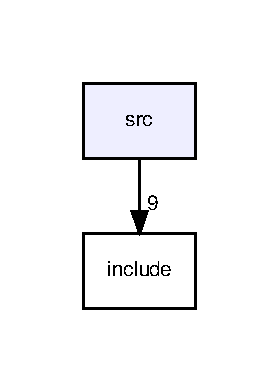
\includegraphics[width=134pt]{dir_8825dd29552366a97c79ae3282986fe7_dep}
\end{center}
\end{figure}
\subsection*{Dateien}
\begin{DoxyCompactItemize}
\item 
Datei \hyperlink{bottom__follow__tag_8cpp}{bottom\_\-follow\_\-tag.cpp}


\begin{DoxyCompactList}\small\item\em Applikation zur Tagvervolgung mit der unteren Kamera. \end{DoxyCompactList}

\item 
Datei \hyperlink{_delta_8cpp}{Delta.cpp}
\item 
Datei \hyperlink{follow__line_8cpp}{follow\_\-line.cpp}


\begin{DoxyCompactList}\small\item\em Applikation zur Linienverfolgung mit der unteren Kamera. \end{DoxyCompactList}

\item 
Datei \hyperlink{front__follow__tag_8cpp}{front\_\-follow\_\-tag.cpp}


\begin{DoxyCompactList}\small\item\em Applikation zur Tagvervolgung mit der vorderen Kamera. \end{DoxyCompactList}

\item 
Datei \hyperlink{_global_8cpp}{Global.cpp}
\item 
Datei \hyperlink{_keyboard_8cpp}{Keyboard.cpp}
\item 
Datei \hyperlink{_log_8cpp}{Log.cpp}
\item 
Datei \hyperlink{_math_8cpp}{Math.cpp}
\end{DoxyCompactItemize}

\chapter{Dokumentation der Namensbereiche}
\hypertarget{namespaceanonymous__namespace_02_math_8cpp_03}{
\section{anonymous\_\-namespace\{Math.cpp\}-\/Namensbereichsreferenz}
\label{namespaceanonymous__namespace_02_math_8cpp_03}\index{anonymous\_\-namespace\{Math.cpp\}@{anonymous\_\-namespace\{Math.cpp\}}}
}
\subsection*{Funktionen}
\begin{DoxyCompactItemize}
\item 
void \hyperlink{namespaceanonymous__namespace_02_math_8cpp_03_af32b12f59241277b0b94ca38ca1d5a4b}{center} (const ar\_\-recog::Tag \&tag, float \&cx, float \&cy, float dx, float dy, float width, float height)
\end{DoxyCompactItemize}


\subsection{Dokumentation der Funktionen}
\hypertarget{namespaceanonymous__namespace_02_math_8cpp_03_af32b12f59241277b0b94ca38ca1d5a4b}{
\index{anonymous\_\-namespace\{Math.cpp\}@{anonymous\_\-namespace\{Math.cpp\}}!center@{center}}
\index{center@{center}!anonymous_namespace{Math.cpp}@{anonymous\_\-namespace\{Math.cpp\}}}
\subsubsection[{center}]{\setlength{\rightskip}{0pt plus 5cm}void anonymous\_\-namespace\{Math.cpp\}::center (
\begin{DoxyParamCaption}
\item[{const ar\_\-recog::Tag \&}]{tag, }
\item[{float \&}]{cx, }
\item[{float \&}]{cy, }
\item[{float}]{dx, }
\item[{float}]{dy, }
\item[{float}]{width, }
\item[{float}]{height}
\end{DoxyParamCaption}
)}}
\label{namespaceanonymous__namespace_02_math_8cpp_03_af32b12f59241277b0b94ca38ca1d5a4b}


Hier ist ein Graph der zeigt, wo diese Funktion aufgerufen wird:\nopagebreak
\begin{figure}[H]
\begin{center}
\leavevmode
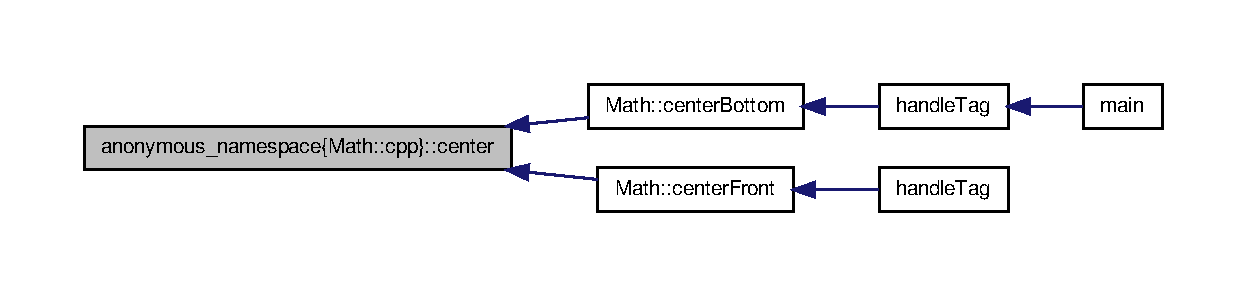
\includegraphics[width=400pt]{namespaceanonymous__namespace_02_math_8cpp_03_af32b12f59241277b0b94ca38ca1d5a4b_icgraph}
\end{center}
\end{figure}



\hypertarget{namespace_keyboard}{
\section{Keyboard-\/Namensbereichsreferenz}
\label{namespace_keyboard}\index{Keyboard@{Keyboard}}
}


enthält \hyperlink{namespace_keyboard_abfb3168172d115a6516147c6d42f58db}{Keyboard::control()} zum steuern der Drone mit der Tastatur  


\subsection*{Funktionen}
\begin{DoxyCompactItemize}
\item 
void \hyperlink{namespace_keyboard_abfb3168172d115a6516147c6d42f58db}{control} ()
\begin{DoxyCompactList}\small\item\em zum Steuern der Drone mit der Tastatur \end{DoxyCompactList}\item 
void \hyperlink{namespace_keyboard_aef945e5d33422ac6abbb326b5203eb5b}{reset\_\-terminal\_\-mode} ()
\item 
void \hyperlink{namespace_keyboard_a6cc4fc3f7daf5630d0570f9d9d21d19c}{set\_\-conio\_\-terminal\_\-mode} ()
\item 
int \hyperlink{namespace_keyboard_a8c142c603571175e17a83a9b99d00d63}{kbhit} ()
\begin{DoxyCompactList}\small\item\em gibt zurück, ob eine Taste gedrückt wurde \end{DoxyCompactList}\item 
int \hyperlink{namespace_keyboard_a433fc58fb356fe62305e8419dd7b33d6}{getch} ()
\begin{DoxyCompactList}\small\item\em gibt zurück, welche Taste gedrückt wurde \end{DoxyCompactList}\end{DoxyCompactItemize}
\subsection*{Variablen}
\begin{DoxyCompactItemize}
\item 
struct termios \hyperlink{namespace_keyboard_a8b623d5192e406c97c4e265dbe4c5f38}{orig\_\-termios}
\end{DoxyCompactItemize}


\subsection{Ausführliche Beschreibung}
enthält \hyperlink{namespace_keyboard_abfb3168172d115a6516147c6d42f58db}{Keyboard::control()} zum steuern der Drone mit der Tastatur 

\subsection{Dokumentation der Funktionen}
\hypertarget{namespace_keyboard_abfb3168172d115a6516147c6d42f58db}{
\index{Keyboard@{Keyboard}!control@{control}}
\index{control@{control}!Keyboard@{Keyboard}}
\subsubsection[{control}]{\setlength{\rightskip}{0pt plus 5cm}void Keyboard::control (
\begin{DoxyParamCaption}
{}
\end{DoxyParamCaption}
)}}
\label{namespace_keyboard_abfb3168172d115a6516147c6d42f58db}


zum Steuern der Drone mit der Tastatur 

muss periodisch aufgerufen werden

w,s,a,d : vorne, hinten, links, rechts

q: nach links drehen

e: nach rechts drehen

o: nach oben fliegen

l: nach unten fliegen

u: um 10\% schneller werden

j: um 10\% langsamer werden 

Hier ist ein Graph der zeigt, was diese Funktion aufruft:\nopagebreak
\begin{figure}[H]
\begin{center}
\leavevmode
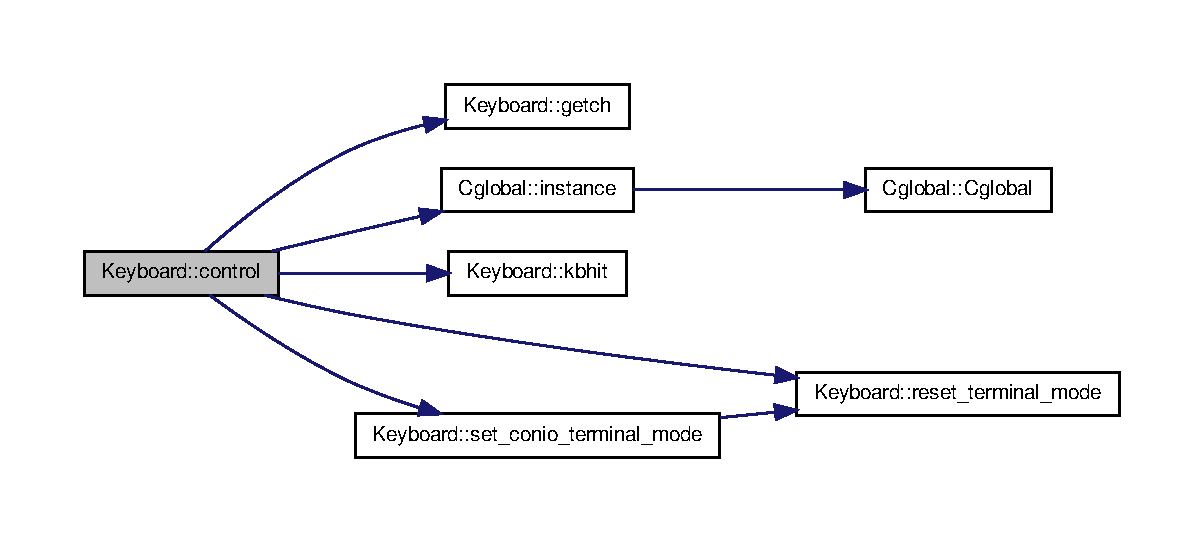
\includegraphics[width=400pt]{namespace_keyboard_abfb3168172d115a6516147c6d42f58db_cgraph}
\end{center}
\end{figure}


\hypertarget{namespace_keyboard_a433fc58fb356fe62305e8419dd7b33d6}{
\index{Keyboard@{Keyboard}!getch@{getch}}
\index{getch@{getch}!Keyboard@{Keyboard}}
\subsubsection[{getch}]{\setlength{\rightskip}{0pt plus 5cm}int Keyboard::getch (
\begin{DoxyParamCaption}
{}
\end{DoxyParamCaption}
)}}
\label{namespace_keyboard_a433fc58fb356fe62305e8419dd7b33d6}


gibt zurück, welche Taste gedrückt wurde 



Hier ist ein Graph der zeigt, wo diese Funktion aufgerufen wird:\nopagebreak
\begin{figure}[H]
\begin{center}
\leavevmode
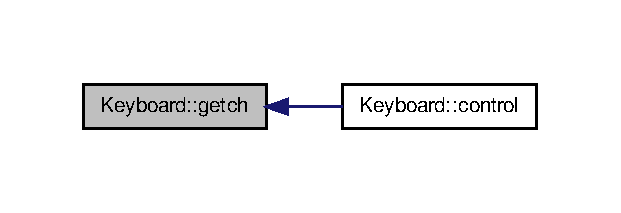
\includegraphics[width=298pt]{namespace_keyboard_a433fc58fb356fe62305e8419dd7b33d6_icgraph}
\end{center}
\end{figure}


\hypertarget{namespace_keyboard_a8c142c603571175e17a83a9b99d00d63}{
\index{Keyboard@{Keyboard}!kbhit@{kbhit}}
\index{kbhit@{kbhit}!Keyboard@{Keyboard}}
\subsubsection[{kbhit}]{\setlength{\rightskip}{0pt plus 5cm}int Keyboard::kbhit (
\begin{DoxyParamCaption}
{}
\end{DoxyParamCaption}
)}}
\label{namespace_keyboard_a8c142c603571175e17a83a9b99d00d63}


gibt zurück, ob eine Taste gedrückt wurde 



Hier ist ein Graph der zeigt, wo diese Funktion aufgerufen wird:\nopagebreak
\begin{figure}[H]
\begin{center}
\leavevmode
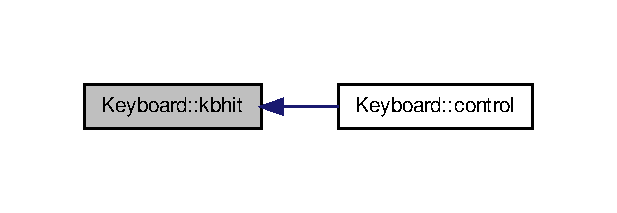
\includegraphics[width=296pt]{namespace_keyboard_a8c142c603571175e17a83a9b99d00d63_icgraph}
\end{center}
\end{figure}


\hypertarget{namespace_keyboard_aef945e5d33422ac6abbb326b5203eb5b}{
\index{Keyboard@{Keyboard}!reset\_\-terminal\_\-mode@{reset\_\-terminal\_\-mode}}
\index{reset\_\-terminal\_\-mode@{reset\_\-terminal\_\-mode}!Keyboard@{Keyboard}}
\subsubsection[{reset\_\-terminal\_\-mode}]{\setlength{\rightskip}{0pt plus 5cm}void Keyboard::reset\_\-terminal\_\-mode (
\begin{DoxyParamCaption}
{}
\end{DoxyParamCaption}
)}}
\label{namespace_keyboard_aef945e5d33422ac6abbb326b5203eb5b}


Hier ist ein Graph der zeigt, wo diese Funktion aufgerufen wird:\nopagebreak
\begin{figure}[H]
\begin{center}
\leavevmode
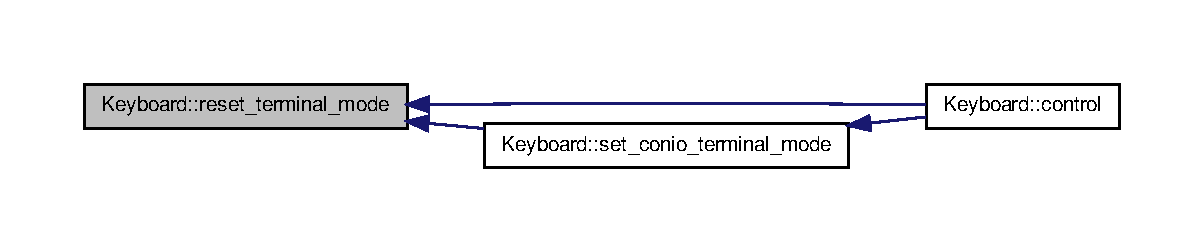
\includegraphics[width=400pt]{namespace_keyboard_aef945e5d33422ac6abbb326b5203eb5b_icgraph}
\end{center}
\end{figure}


\hypertarget{namespace_keyboard_a6cc4fc3f7daf5630d0570f9d9d21d19c}{
\index{Keyboard@{Keyboard}!set\_\-conio\_\-terminal\_\-mode@{set\_\-conio\_\-terminal\_\-mode}}
\index{set\_\-conio\_\-terminal\_\-mode@{set\_\-conio\_\-terminal\_\-mode}!Keyboard@{Keyboard}}
\subsubsection[{set\_\-conio\_\-terminal\_\-mode}]{\setlength{\rightskip}{0pt plus 5cm}void Keyboard::set\_\-conio\_\-terminal\_\-mode (
\begin{DoxyParamCaption}
{}
\end{DoxyParamCaption}
)}}
\label{namespace_keyboard_a6cc4fc3f7daf5630d0570f9d9d21d19c}


Hier ist ein Graph der zeigt, was diese Funktion aufruft:\nopagebreak
\begin{figure}[H]
\begin{center}
\leavevmode
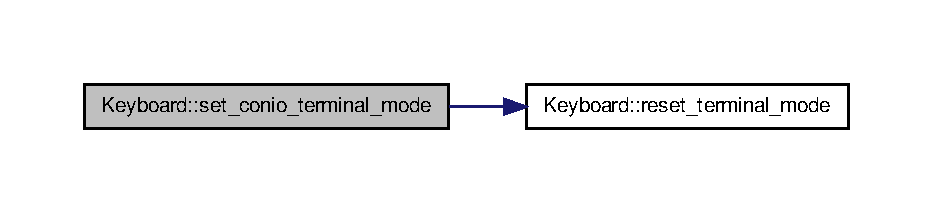
\includegraphics[width=400pt]{namespace_keyboard_a6cc4fc3f7daf5630d0570f9d9d21d19c_cgraph}
\end{center}
\end{figure}




Hier ist ein Graph der zeigt, wo diese Funktion aufgerufen wird:\nopagebreak
\begin{figure}[H]
\begin{center}
\leavevmode
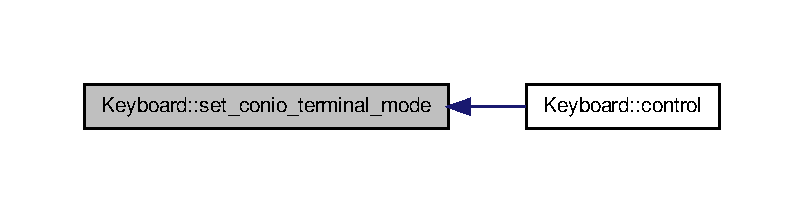
\includegraphics[width=386pt]{namespace_keyboard_a6cc4fc3f7daf5630d0570f9d9d21d19c_icgraph}
\end{center}
\end{figure}




\subsection{Variablen-\/Dokumentation}
\hypertarget{namespace_keyboard_a8b623d5192e406c97c4e265dbe4c5f38}{
\index{Keyboard@{Keyboard}!orig\_\-termios@{orig\_\-termios}}
\index{orig\_\-termios@{orig\_\-termios}!Keyboard@{Keyboard}}
\subsubsection[{orig\_\-termios}]{\setlength{\rightskip}{0pt plus 5cm}struct termios {\bf Keyboard::orig\_\-termios}}}
\label{namespace_keyboard_a8b623d5192e406c97c4e265dbe4c5f38}

\hypertarget{namespace_math}{
\section{Math-\/Namensbereichsreferenz}
\label{namespace_math}\index{Math@{Math}}
}
\subsection*{Funktionen}
\begin{DoxyCompactItemize}
\item 
void \hyperlink{namespace_math_a25b9284eb485b732c952786b63343aaa}{pixelDiffBottom} (float \&x, float \&y)
\begin{DoxyCompactList}\small\item\em Berechnung der Anzahl der Pixel für die Frontkamera, um die das Tag aufgrund der Rotation verschoben wurde. \end{DoxyCompactList}\item 
void \hyperlink{namespace_math_a3fbe7036db847d74ed5f2c21635d02d9}{pixelDiffFront} (float \&x, float \&y)
\item 
void \hyperlink{namespace_math_ab4c584467f0cc5d8af22a69482630866}{centerBottom} (const ar\_\-recog::Tag \&tag, float \&cx, float \&cy)
\begin{DoxyCompactList}\small\item\em Berechnung aus den Eckpunkten wo sich das Tag bezüglich des Bildes befindet. \end{DoxyCompactList}\item 
void \hyperlink{namespace_math_a43f025fac1ade5dbf88f7c393ca85644}{centerFront} (const ar\_\-recog::Tag \&tag, float \&cx, float \&cy)
\item 
void \hyperlink{namespace_math_ad3b65f0aedda56076f681f2b987d0e5c}{navdataUpdate} (const ardrone\_\-brown::Navdata::ConstPtr \&navdata)
\begin{DoxyCompactList}\small\item\em subscriber handler für die Nachricht /ardrone/navdata \end{DoxyCompactList}\end{DoxyCompactItemize}


\subsection{Dokumentation der Funktionen}
\hypertarget{namespace_math_ab4c584467f0cc5d8af22a69482630866}{
\index{Math@{Math}!centerBottom@{centerBottom}}
\index{centerBottom@{centerBottom}!Math@{Math}}
\subsubsection[{centerBottom}]{\setlength{\rightskip}{0pt plus 5cm}void Math::centerBottom (
\begin{DoxyParamCaption}
\item[{const ar\_\-recog::Tag \&}]{tag, }
\item[{float \&}]{cx, }
\item[{float \&}]{cy}
\end{DoxyParamCaption}
)}}
\label{namespace_math_ab4c584467f0cc5d8af22a69482630866}


Berechnung aus den Eckpunkten wo sich das Tag bezüglich des Bildes befindet. 

cy: 0 Tag ist am oberen Bildrand, 0.5 Tag ist in der Mitte(Höhe), 1 Tag ist am unteren Bildrand cx: 0 Tag ist am linken Bildrand, 0.5 Tag ist in der Mitte(Breite), 1 Tag ist am rechten Bildrend 

Hier ist ein Graph der zeigt, was diese Funktion aufruft:\nopagebreak
\begin{figure}[H]
\begin{center}
\leavevmode
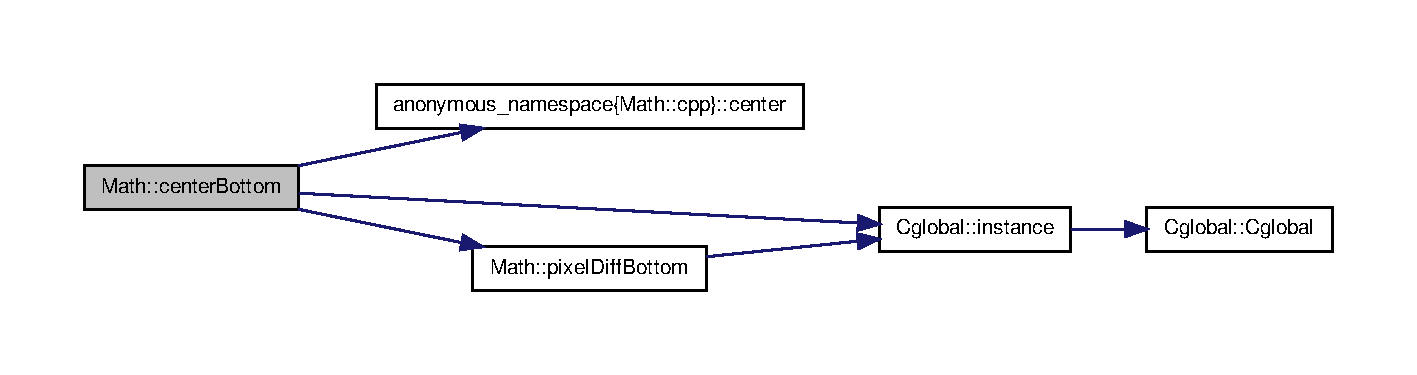
\includegraphics[width=400pt]{namespace_math_ab4c584467f0cc5d8af22a69482630866_cgraph}
\end{center}
\end{figure}




Hier ist ein Graph der zeigt, wo diese Funktion aufgerufen wird:\nopagebreak
\begin{figure}[H]
\begin{center}
\leavevmode
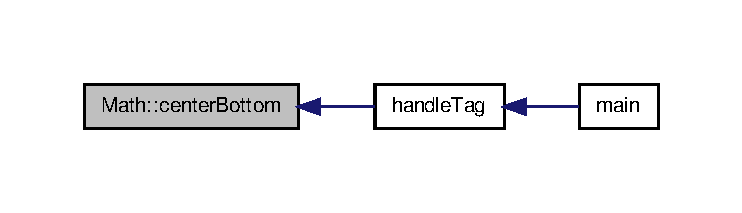
\includegraphics[width=356pt]{namespace_math_ab4c584467f0cc5d8af22a69482630866_icgraph}
\end{center}
\end{figure}


\hypertarget{namespace_math_a43f025fac1ade5dbf88f7c393ca85644}{
\index{Math@{Math}!centerFront@{centerFront}}
\index{centerFront@{centerFront}!Math@{Math}}
\subsubsection[{centerFront}]{\setlength{\rightskip}{0pt plus 5cm}void Math::centerFront (
\begin{DoxyParamCaption}
\item[{const ar\_\-recog::Tag \&}]{tag, }
\item[{float \&}]{cx, }
\item[{float \&}]{cy}
\end{DoxyParamCaption}
)}}
\label{namespace_math_a43f025fac1ade5dbf88f7c393ca85644}


Hier ist ein Graph der zeigt, was diese Funktion aufruft:\nopagebreak
\begin{figure}[H]
\begin{center}
\leavevmode
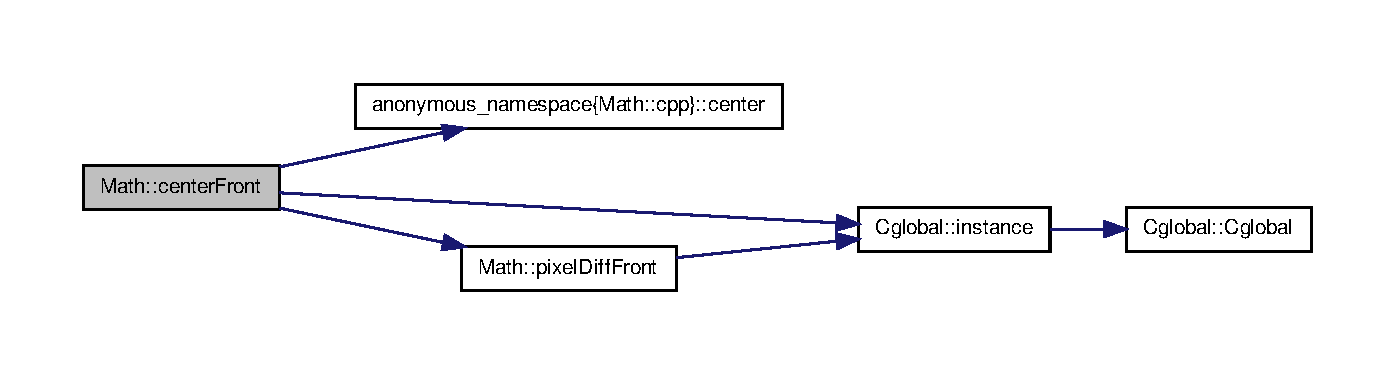
\includegraphics[width=400pt]{namespace_math_a43f025fac1ade5dbf88f7c393ca85644_cgraph}
\end{center}
\end{figure}




Hier ist ein Graph der zeigt, wo diese Funktion aufgerufen wird:\nopagebreak
\begin{figure}[H]
\begin{center}
\leavevmode
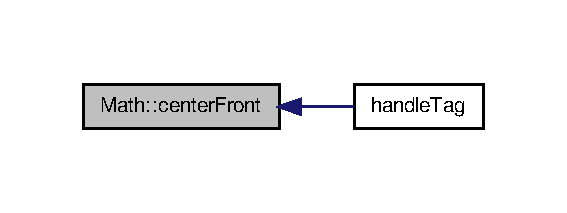
\includegraphics[width=272pt]{namespace_math_a43f025fac1ade5dbf88f7c393ca85644_icgraph}
\end{center}
\end{figure}


\hypertarget{namespace_math_ad3b65f0aedda56076f681f2b987d0e5c}{
\index{Math@{Math}!navdataUpdate@{navdataUpdate}}
\index{navdataUpdate@{navdataUpdate}!Math@{Math}}
\subsubsection[{navdataUpdate}]{\setlength{\rightskip}{0pt plus 5cm}void Math::navdataUpdate (
\begin{DoxyParamCaption}
\item[{const ardrone\_\-brown::Navdata::ConstPtr \&}]{navdata}
\end{DoxyParamCaption}
)}}
\label{namespace_math_ad3b65f0aedda56076f681f2b987d0e5c}


subscriber handler für die Nachricht /ardrone/navdata 

speichert die Navdata-\/Informationen 

Hier ist ein Graph der zeigt, was diese Funktion aufruft:\nopagebreak
\begin{figure}[H]
\begin{center}
\leavevmode
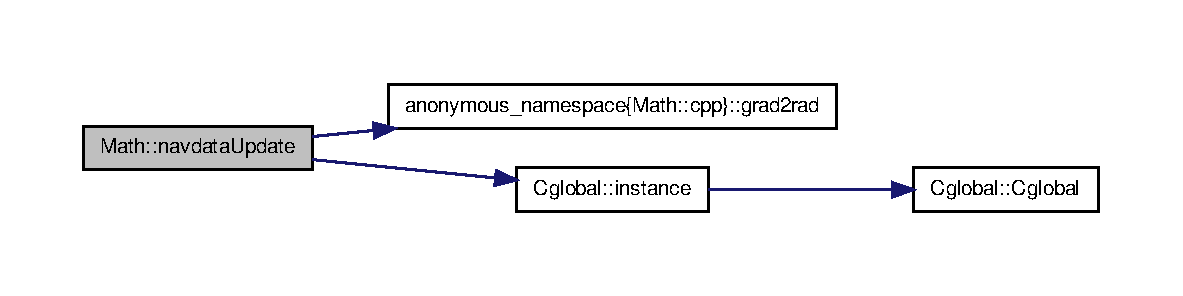
\includegraphics[width=400pt]{namespace_math_ad3b65f0aedda56076f681f2b987d0e5c_cgraph}
\end{center}
\end{figure}




Hier ist ein Graph der zeigt, wo diese Funktion aufgerufen wird:\nopagebreak
\begin{figure}[H]
\begin{center}
\leavevmode
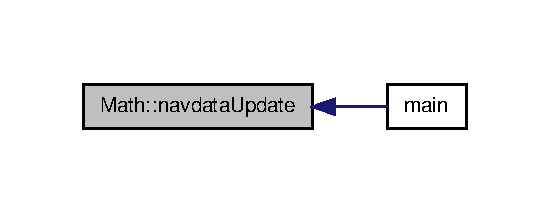
\includegraphics[width=264pt]{namespace_math_ad3b65f0aedda56076f681f2b987d0e5c_icgraph}
\end{center}
\end{figure}


\hypertarget{namespace_math_a25b9284eb485b732c952786b63343aaa}{
\index{Math@{Math}!pixelDiffBottom@{pixelDiffBottom}}
\index{pixelDiffBottom@{pixelDiffBottom}!Math@{Math}}
\subsubsection[{pixelDiffBottom}]{\setlength{\rightskip}{0pt plus 5cm}void Math::pixelDiffBottom (
\begin{DoxyParamCaption}
\item[{float \&}]{x, }
\item[{float \&}]{y}
\end{DoxyParamCaption}
)}}
\label{namespace_math_a25b9284eb485b732c952786b63343aaa}


Berechnung der Anzahl der Pixel für die Frontkamera, um die das Tag aufgrund der Rotation verschoben wurde. 

Problem: Sichtfeld ist noch nicht korrekt berechnet(derzeit für x und y Richtung gleich)


\begin{DoxyParams}{Parameter}
{\em x} & Verschiebung in x Richung \\
\hline
{\em y} & Verschiebung in y Richung\\
\hline
\end{DoxyParams}
 

Hier ist ein Graph der zeigt, was diese Funktion aufruft:\nopagebreak
\begin{figure}[H]
\begin{center}
\leavevmode
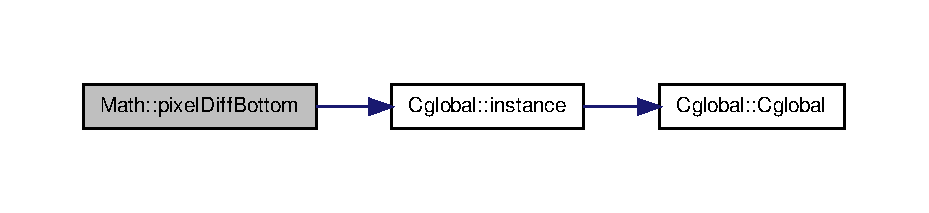
\includegraphics[width=400pt]{namespace_math_a25b9284eb485b732c952786b63343aaa_cgraph}
\end{center}
\end{figure}




Hier ist ein Graph der zeigt, wo diese Funktion aufgerufen wird:\nopagebreak
\begin{figure}[H]
\begin{center}
\leavevmode
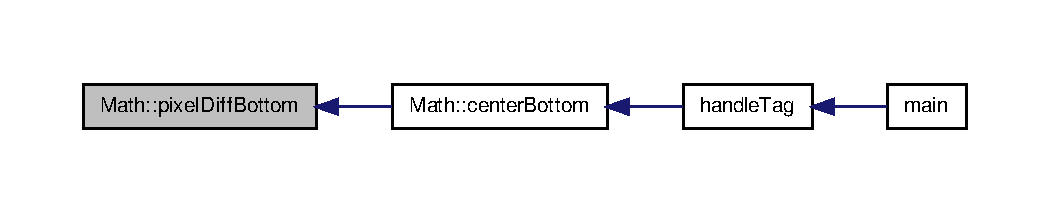
\includegraphics[width=400pt]{namespace_math_a25b9284eb485b732c952786b63343aaa_icgraph}
\end{center}
\end{figure}


\hypertarget{namespace_math_a3fbe7036db847d74ed5f2c21635d02d9}{
\index{Math@{Math}!pixelDiffFront@{pixelDiffFront}}
\index{pixelDiffFront@{pixelDiffFront}!Math@{Math}}
\subsubsection[{pixelDiffFront}]{\setlength{\rightskip}{0pt plus 5cm}void Math::pixelDiffFront (
\begin{DoxyParamCaption}
\item[{float \&}]{x, }
\item[{float \&}]{y}
\end{DoxyParamCaption}
)}}
\label{namespace_math_a3fbe7036db847d74ed5f2c21635d02d9}


Hier ist ein Graph der zeigt, was diese Funktion aufruft:\nopagebreak
\begin{figure}[H]
\begin{center}
\leavevmode
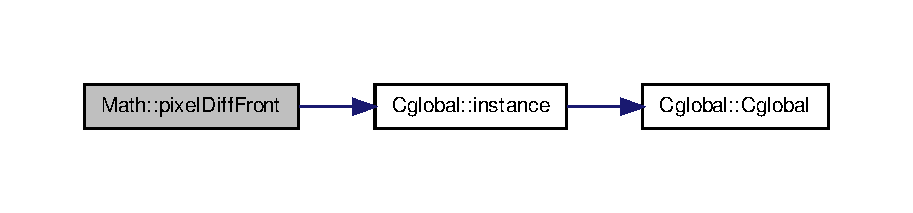
\includegraphics[width=400pt]{namespace_math_a3fbe7036db847d74ed5f2c21635d02d9_cgraph}
\end{center}
\end{figure}




Hier ist ein Graph der zeigt, wo diese Funktion aufgerufen wird:\nopagebreak
\begin{figure}[H]
\begin{center}
\leavevmode
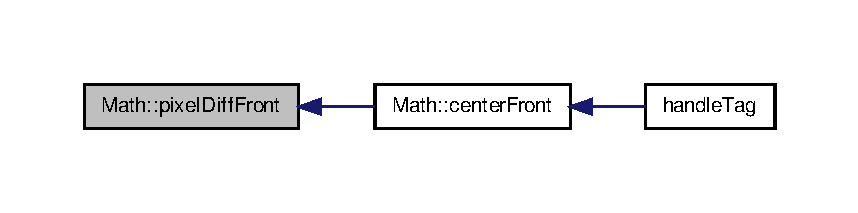
\includegraphics[width=400pt]{namespace_math_a3fbe7036db847d74ed5f2c21635d02d9_icgraph}
\end{center}
\end{figure}



\chapter{Klassen-\/Dokumentation}
\hypertarget{class_cglobal}{
\section{Cglobal Klassenreferenz}
\label{class_cglobal}\index{Cglobal@{Cglobal}}
}


{\ttfamily \#include $<$Global.h$>$}



Zusammengehörigkeiten von Cglobal:\nopagebreak
\begin{figure}[H]
\begin{center}
\leavevmode
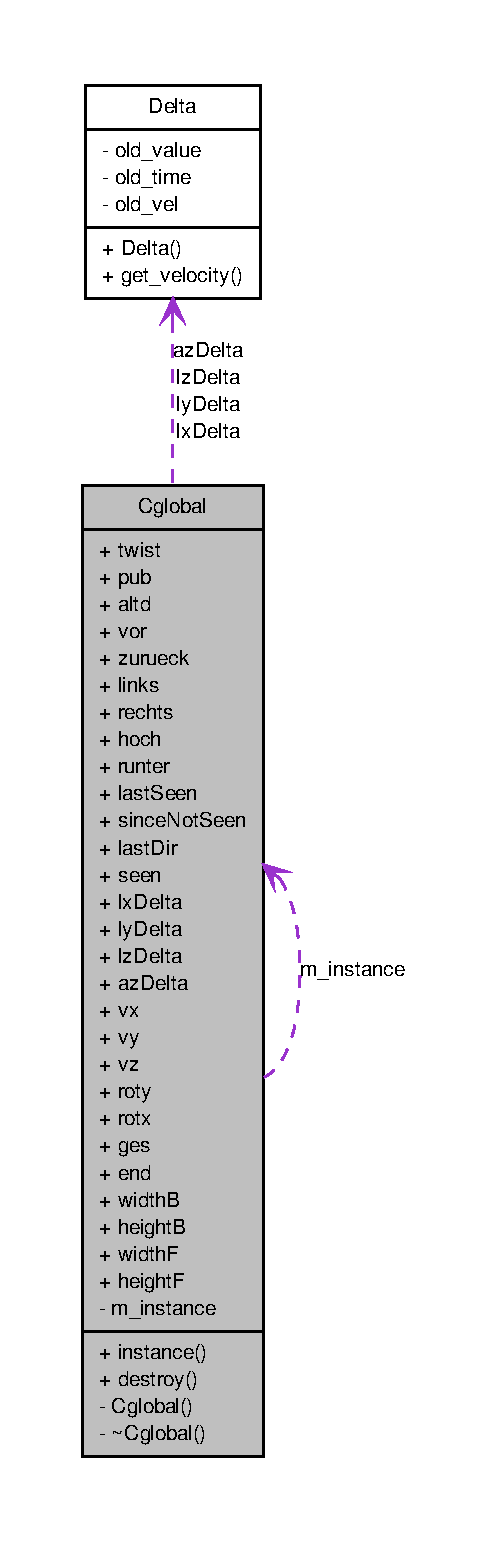
\includegraphics[height=600pt]{class_cglobal__coll__graph}
\end{center}
\end{figure}
\subsection*{Öffentliche, statische Methoden}
\begin{DoxyCompactItemize}
\item 
static \hyperlink{class_cglobal}{Cglobal} \& \hyperlink{class_cglobal_a0e96a5f7f00ef5a151da708a17340f08}{instance} ()
\item 
static void \hyperlink{class_cglobal_aa1d07161425d12bc42dd100140407e59}{destroy} ()
\end{DoxyCompactItemize}
\subsection*{Öffentliche Attribute}
\begin{DoxyCompactItemize}
\item 
geometry\_\-msgs::Twist \hyperlink{class_cglobal_acdd49b2fad30faf04785664c422f5ef7}{twist}
\begin{DoxyCompactList}\small\item\em Zur Ansteuerung der Drone. \end{DoxyCompactList}\item 
ros::Publisher \hyperlink{class_cglobal_af3a06302b3bd19de728064359241c1a1}{pub}
\begin{DoxyCompactList}\small\item\em publisher zum publishen des Twist Objekts \end{DoxyCompactList}\item 
int \hyperlink{class_cglobal_a0e2d4712edf675715bd4bcc554dbcf42}{altd}
\begin{DoxyCompactList}\small\item\em Höhe. \end{DoxyCompactList}\item 
bool \hyperlink{class_cglobal_ac0b3c90a19b5395a404bb9e5aee44e1c}{vor}
\begin{DoxyCompactList}\small\item\em will die Drone nach vorne fliegen? \end{DoxyCompactList}\item 
bool \hyperlink{class_cglobal_a1b0b85d52fea92c819e421db042b704d}{zurueck}
\item 
bool \hyperlink{class_cglobal_a10e812f9c1b4e7b7544b959d1b5f120b}{links}
\item 
bool \hyperlink{class_cglobal_a718da04af5940be1ad811f61b85f57d6}{rechts}
\item 
bool \hyperlink{class_cglobal_a57b8d93cd26f7c778c719ad21bc5528b}{hoch}
\item 
bool \hyperlink{class_cglobal_a3198b29c259c188b0938b4fb5731409b}{runter}
\item 
time\_\-t \hyperlink{class_cglobal_a1d338ed39494adfbee95a883369e5f4a}{lastSeen}
\item 
time\_\-t \hyperlink{class_cglobal_abb1e0f2a241a8d9131098cf823b45f64}{sinceNotSeen}
\item 
float \hyperlink{class_cglobal_a3ab9e8044e12c2927366e5402b5e3c09}{lastDir}
\item 
bool \hyperlink{class_cglobal_afe6f01a7ff64a3de6d0c8612f36511fd}{seen}
\item 
\hyperlink{class_delta}{Delta} \hyperlink{class_cglobal_ae826fb1d5b65ba58163f25517431e505}{lxDelta}
\item 
\hyperlink{class_delta}{Delta} \hyperlink{class_cglobal_a42b74fa677f900102efb348d7189ca3c}{lyDelta}
\item 
\hyperlink{class_delta}{Delta} \hyperlink{class_cglobal_aaff1f24cae62247123759d5142d5f69a}{lzDelta}
\item 
\hyperlink{class_delta}{Delta} \hyperlink{class_cglobal_a4a7fa181ec17c448e6f7ef4d7213789b}{azDelta}
\item 
float \hyperlink{class_cglobal_abafbed62176301706747c04ef3046aae}{vx}
\item 
float \hyperlink{class_cglobal_a0967372a0ede7b8b9a24957df663b7b3}{vy}
\item 
float \hyperlink{class_cglobal_af9ef9759f83ae67b7e220570a7738ef5}{vz}
\item 
float \hyperlink{class_cglobal_a5c1fac565d3813e798bd6aeb1c6fc8aa}{roty}
\item 
float \hyperlink{class_cglobal_ad295728f5113d9a47527cf14262dea0e}{rotx}
\item 
float \hyperlink{class_cglobal_a478c0d94a8f8a7675d3e88e85742c81a}{ges}
\item 
bool \hyperlink{class_cglobal_a24fbb5c4b0ddab650375d08ba677b3f1}{end}
\item 
int \hyperlink{class_cglobal_a3adbbe83dbdab17a3506572de5444d14}{widthB}
\item 
int \hyperlink{class_cglobal_ae1a1fde7d947c2c7d32bc7f76599b054}{heightB}
\item 
int \hyperlink{class_cglobal_add77c33bb751ff75fc5e6bc0409d4540}{widthF}
\item 
int \hyperlink{class_cglobal_ac4dace71dbed15b75354e5ff327af75f}{heightF}
\end{DoxyCompactItemize}
\subsection*{Private Methoden}
\begin{DoxyCompactItemize}
\item 
\hyperlink{class_cglobal_a9847b00476a6f18dbd936472e1a9efbf}{Cglobal} ()
\item 
\hyperlink{class_cglobal_a16a55c21346fe1cd9b9511ee05fd485e}{$\sim$Cglobal} ()
\end{DoxyCompactItemize}
\subsection*{Statische private Attribute}
\begin{DoxyCompactItemize}
\item 
static \hyperlink{class_cglobal}{Cglobal} $\ast$ \hyperlink{class_cglobal_afb7ab45601acda975c029de5db73b3ea}{m\_\-instance} = 0
\end{DoxyCompactItemize}


\subsection{Beschreibung der Konstruktoren und Destruktoren}
\hypertarget{class_cglobal_a9847b00476a6f18dbd936472e1a9efbf}{
\index{Cglobal@{Cglobal}!Cglobal@{Cglobal}}
\index{Cglobal@{Cglobal}!Cglobal@{Cglobal}}
\subsubsection[{Cglobal}]{\setlength{\rightskip}{0pt plus 5cm}Cglobal::Cglobal (
\begin{DoxyParamCaption}
{}
\end{DoxyParamCaption}
)\hspace{0.3cm}{\ttfamily  \mbox{[}private\mbox{]}}}}
\label{class_cglobal_a9847b00476a6f18dbd936472e1a9efbf}


Hier ist ein Graph der zeigt, wo diese Funktion aufgerufen wird:
\nopagebreak
\begin{figure}[H]
\begin{center}
\leavevmode
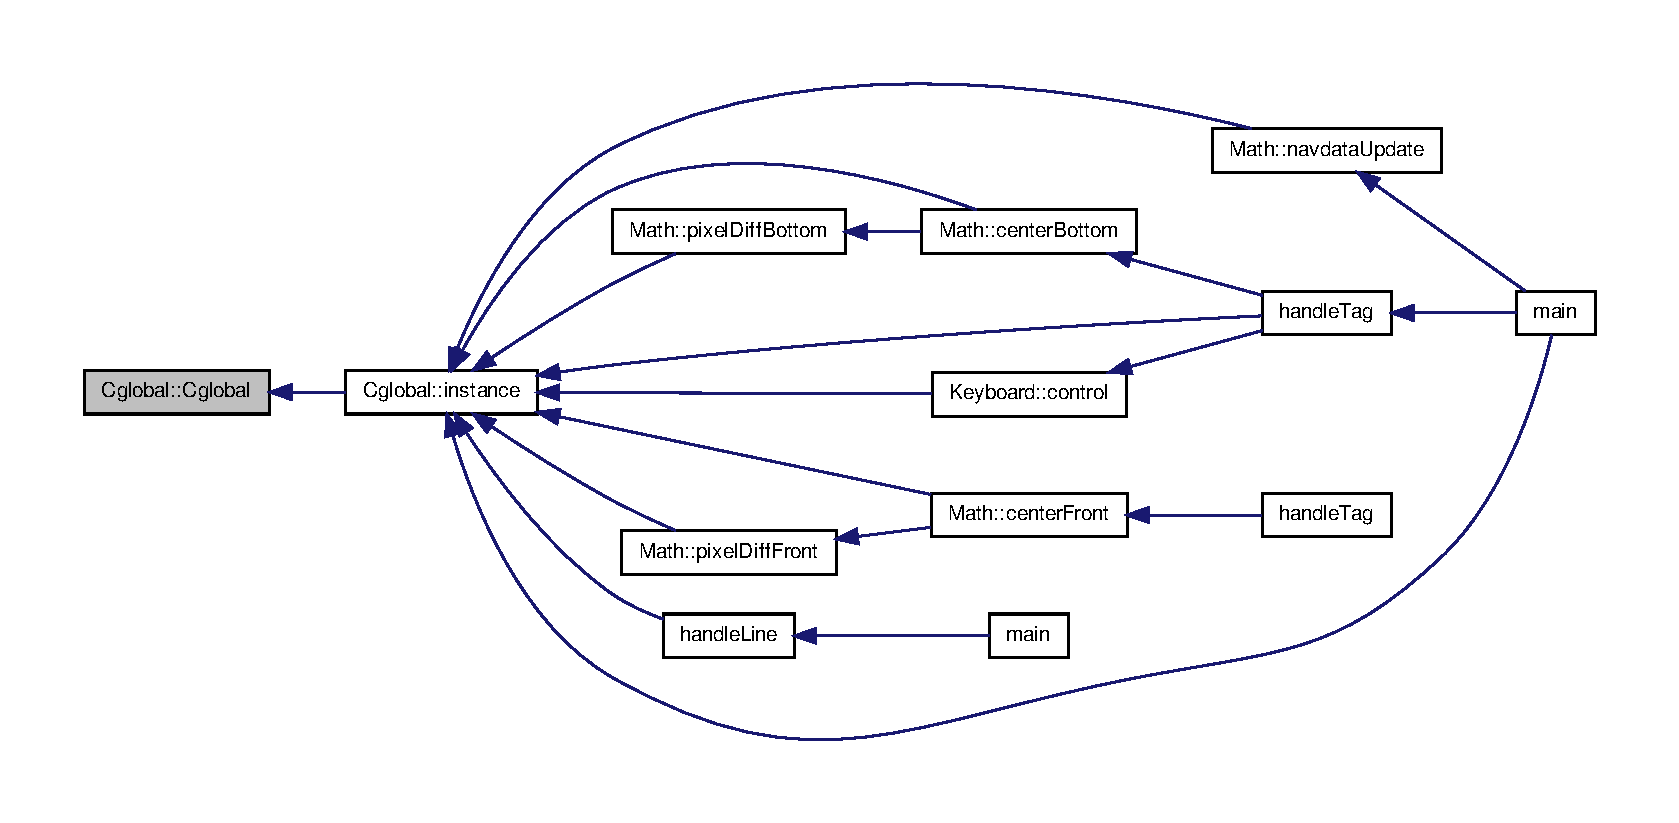
\includegraphics[width=400pt]{class_cglobal_a9847b00476a6f18dbd936472e1a9efbf_icgraph}
\end{center}
\end{figure}


\hypertarget{class_cglobal_a16a55c21346fe1cd9b9511ee05fd485e}{
\index{Cglobal@{Cglobal}!$\sim$Cglobal@{$\sim$Cglobal}}
\index{$\sim$Cglobal@{$\sim$Cglobal}!Cglobal@{Cglobal}}
\subsubsection[{$\sim$Cglobal}]{\setlength{\rightskip}{0pt plus 5cm}Cglobal::$\sim$Cglobal (
\begin{DoxyParamCaption}
{}
\end{DoxyParamCaption}
)\hspace{0.3cm}{\ttfamily  \mbox{[}inline, private\mbox{]}}}}
\label{class_cglobal_a16a55c21346fe1cd9b9511ee05fd485e}


\subsection{Dokumentation der Elementfunktionen}
\hypertarget{class_cglobal_aa1d07161425d12bc42dd100140407e59}{
\index{Cglobal@{Cglobal}!destroy@{destroy}}
\index{destroy@{destroy}!Cglobal@{Cglobal}}
\subsubsection[{destroy}]{\setlength{\rightskip}{0pt plus 5cm}void Cglobal::destroy (
\begin{DoxyParamCaption}
{}
\end{DoxyParamCaption}
)\hspace{0.3cm}{\ttfamily  \mbox{[}static\mbox{]}}}}
\label{class_cglobal_aa1d07161425d12bc42dd100140407e59}


Hier ist ein Graph der zeigt, wo diese Funktion aufgerufen wird:\nopagebreak
\begin{figure}[H]
\begin{center}
\leavevmode
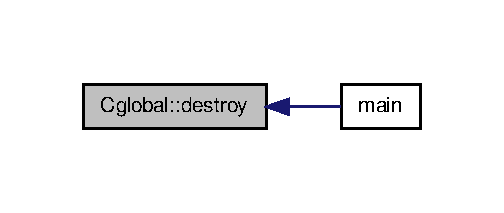
\includegraphics[width=242pt]{class_cglobal_aa1d07161425d12bc42dd100140407e59_icgraph}
\end{center}
\end{figure}


\hypertarget{class_cglobal_a0e96a5f7f00ef5a151da708a17340f08}{
\index{Cglobal@{Cglobal}!instance@{instance}}
\index{instance@{instance}!Cglobal@{Cglobal}}
\subsubsection[{instance}]{\setlength{\rightskip}{0pt plus 5cm}{\bf Cglobal} \& Cglobal::instance (
\begin{DoxyParamCaption}
{}
\end{DoxyParamCaption}
)\hspace{0.3cm}{\ttfamily  \mbox{[}static\mbox{]}}}}
\label{class_cglobal_a0e96a5f7f00ef5a151da708a17340f08}


Hier ist ein Graph der zeigt, was diese Funktion aufruft:\nopagebreak
\begin{figure}[H]
\begin{center}
\leavevmode
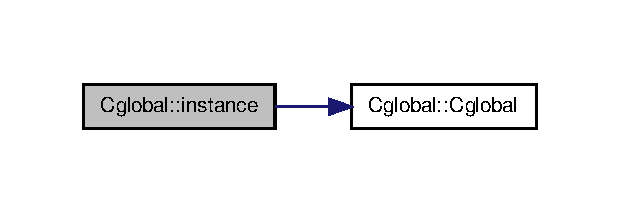
\includegraphics[width=298pt]{class_cglobal_a0e96a5f7f00ef5a151da708a17340f08_cgraph}
\end{center}
\end{figure}




Hier ist ein Graph der zeigt, wo diese Funktion aufgerufen wird:
\nopagebreak
\begin{figure}[H]
\begin{center}
\leavevmode
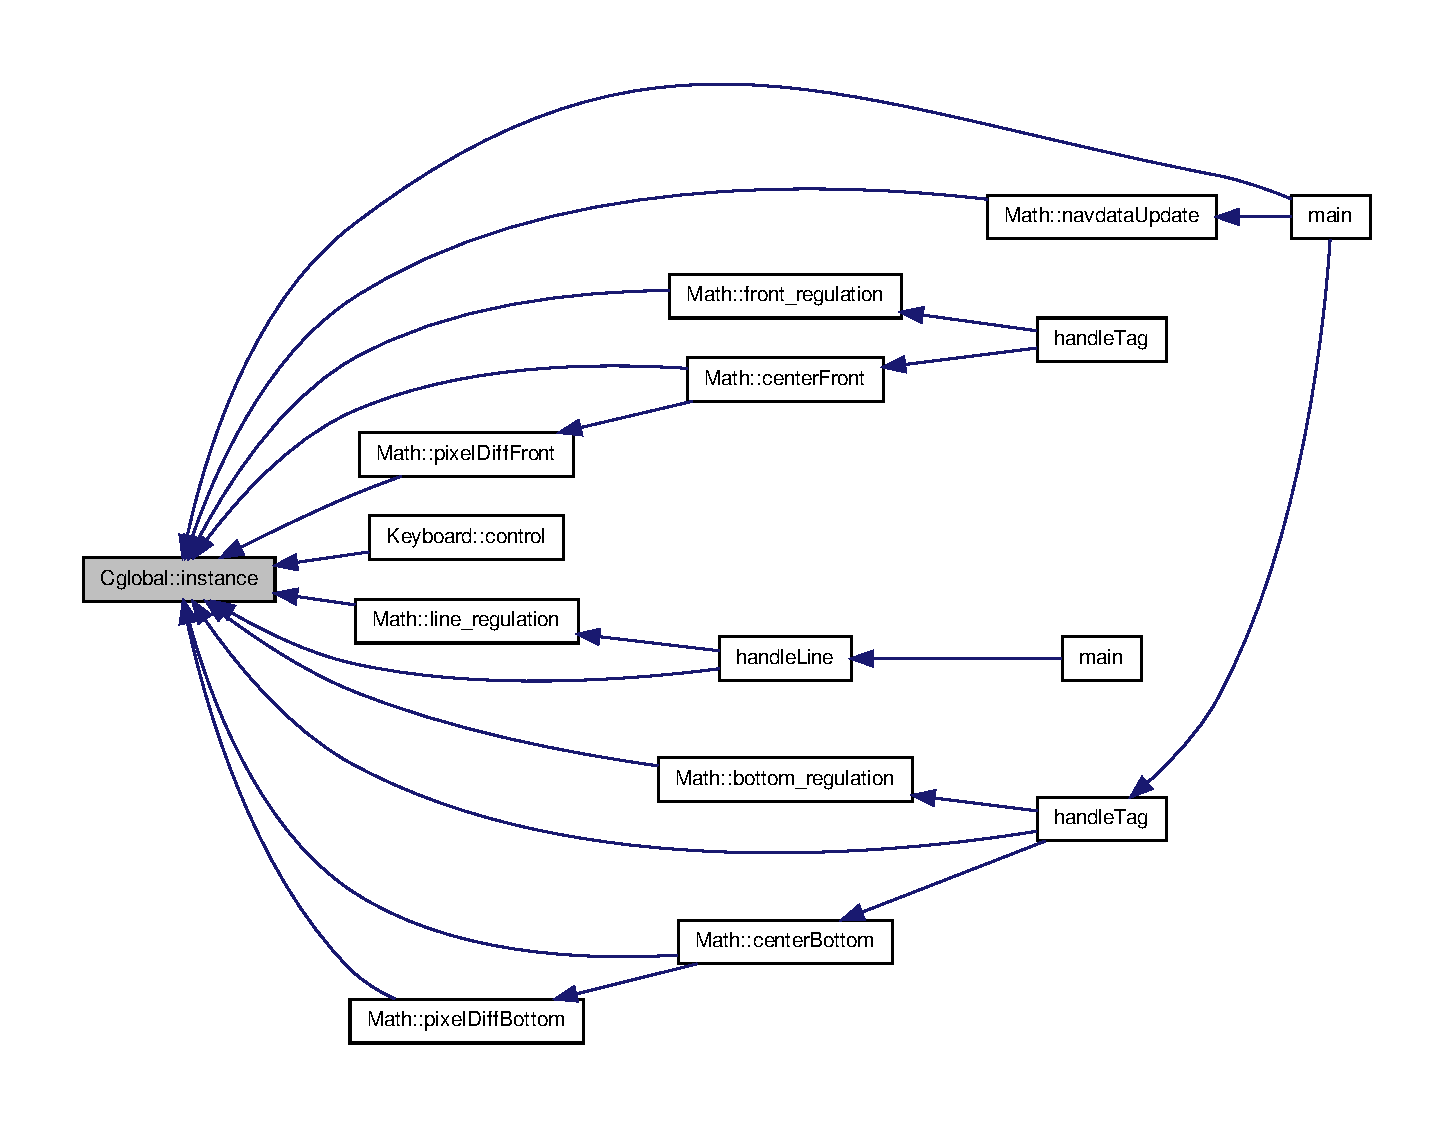
\includegraphics[width=400pt]{class_cglobal_a0e96a5f7f00ef5a151da708a17340f08_icgraph}
\end{center}
\end{figure}




\subsection{Dokumentation der Datenelemente}
\hypertarget{class_cglobal_a0e2d4712edf675715bd4bcc554dbcf42}{
\index{Cglobal@{Cglobal}!altd@{altd}}
\index{altd@{altd}!Cglobal@{Cglobal}}
\subsubsection[{altd}]{\setlength{\rightskip}{0pt plus 5cm}int {\bf Cglobal::altd}}}
\label{class_cglobal_a0e2d4712edf675715bd4bcc554dbcf42}


Höhe. 

\hypertarget{class_cglobal_a4a7fa181ec17c448e6f7ef4d7213789b}{
\index{Cglobal@{Cglobal}!azDelta@{azDelta}}
\index{azDelta@{azDelta}!Cglobal@{Cglobal}}
\subsubsection[{azDelta}]{\setlength{\rightskip}{0pt plus 5cm}{\bf Delta} {\bf Cglobal::azDelta}}}
\label{class_cglobal_a4a7fa181ec17c448e6f7ef4d7213789b}
\hypertarget{class_cglobal_a24fbb5c4b0ddab650375d08ba677b3f1}{
\index{Cglobal@{Cglobal}!end@{end}}
\index{end@{end}!Cglobal@{Cglobal}}
\subsubsection[{end}]{\setlength{\rightskip}{0pt plus 5cm}bool {\bf Cglobal::end}}}
\label{class_cglobal_a24fbb5c4b0ddab650375d08ba677b3f1}
\hypertarget{class_cglobal_a478c0d94a8f8a7675d3e88e85742c81a}{
\index{Cglobal@{Cglobal}!ges@{ges}}
\index{ges@{ges}!Cglobal@{Cglobal}}
\subsubsection[{ges}]{\setlength{\rightskip}{0pt plus 5cm}float {\bf Cglobal::ges}}}
\label{class_cglobal_a478c0d94a8f8a7675d3e88e85742c81a}
\hypertarget{class_cglobal_ae1a1fde7d947c2c7d32bc7f76599b054}{
\index{Cglobal@{Cglobal}!heightB@{heightB}}
\index{heightB@{heightB}!Cglobal@{Cglobal}}
\subsubsection[{heightB}]{\setlength{\rightskip}{0pt plus 5cm}int {\bf Cglobal::heightB}}}
\label{class_cglobal_ae1a1fde7d947c2c7d32bc7f76599b054}
\hypertarget{class_cglobal_ac4dace71dbed15b75354e5ff327af75f}{
\index{Cglobal@{Cglobal}!heightF@{heightF}}
\index{heightF@{heightF}!Cglobal@{Cglobal}}
\subsubsection[{heightF}]{\setlength{\rightskip}{0pt plus 5cm}int {\bf Cglobal::heightF}}}
\label{class_cglobal_ac4dace71dbed15b75354e5ff327af75f}
\hypertarget{class_cglobal_a57b8d93cd26f7c778c719ad21bc5528b}{
\index{Cglobal@{Cglobal}!hoch@{hoch}}
\index{hoch@{hoch}!Cglobal@{Cglobal}}
\subsubsection[{hoch}]{\setlength{\rightskip}{0pt plus 5cm}bool {\bf Cglobal::hoch}}}
\label{class_cglobal_a57b8d93cd26f7c778c719ad21bc5528b}
\hypertarget{class_cglobal_a3ab9e8044e12c2927366e5402b5e3c09}{
\index{Cglobal@{Cglobal}!lastDir@{lastDir}}
\index{lastDir@{lastDir}!Cglobal@{Cglobal}}
\subsubsection[{lastDir}]{\setlength{\rightskip}{0pt plus 5cm}float {\bf Cglobal::lastDir}}}
\label{class_cglobal_a3ab9e8044e12c2927366e5402b5e3c09}
\hypertarget{class_cglobal_a1d338ed39494adfbee95a883369e5f4a}{
\index{Cglobal@{Cglobal}!lastSeen@{lastSeen}}
\index{lastSeen@{lastSeen}!Cglobal@{Cglobal}}
\subsubsection[{lastSeen}]{\setlength{\rightskip}{0pt plus 5cm}time\_\-t {\bf Cglobal::lastSeen}}}
\label{class_cglobal_a1d338ed39494adfbee95a883369e5f4a}
\hypertarget{class_cglobal_a10e812f9c1b4e7b7544b959d1b5f120b}{
\index{Cglobal@{Cglobal}!links@{links}}
\index{links@{links}!Cglobal@{Cglobal}}
\subsubsection[{links}]{\setlength{\rightskip}{0pt plus 5cm}bool {\bf Cglobal::links}}}
\label{class_cglobal_a10e812f9c1b4e7b7544b959d1b5f120b}
\hypertarget{class_cglobal_ae826fb1d5b65ba58163f25517431e505}{
\index{Cglobal@{Cglobal}!lxDelta@{lxDelta}}
\index{lxDelta@{lxDelta}!Cglobal@{Cglobal}}
\subsubsection[{lxDelta}]{\setlength{\rightskip}{0pt plus 5cm}{\bf Delta} {\bf Cglobal::lxDelta}}}
\label{class_cglobal_ae826fb1d5b65ba58163f25517431e505}
\hypertarget{class_cglobal_a42b74fa677f900102efb348d7189ca3c}{
\index{Cglobal@{Cglobal}!lyDelta@{lyDelta}}
\index{lyDelta@{lyDelta}!Cglobal@{Cglobal}}
\subsubsection[{lyDelta}]{\setlength{\rightskip}{0pt plus 5cm}{\bf Delta} {\bf Cglobal::lyDelta}}}
\label{class_cglobal_a42b74fa677f900102efb348d7189ca3c}
\hypertarget{class_cglobal_aaff1f24cae62247123759d5142d5f69a}{
\index{Cglobal@{Cglobal}!lzDelta@{lzDelta}}
\index{lzDelta@{lzDelta}!Cglobal@{Cglobal}}
\subsubsection[{lzDelta}]{\setlength{\rightskip}{0pt plus 5cm}{\bf Delta} {\bf Cglobal::lzDelta}}}
\label{class_cglobal_aaff1f24cae62247123759d5142d5f69a}
\hypertarget{class_cglobal_afb7ab45601acda975c029de5db73b3ea}{
\index{Cglobal@{Cglobal}!m\_\-instance@{m\_\-instance}}
\index{m\_\-instance@{m\_\-instance}!Cglobal@{Cglobal}}
\subsubsection[{m\_\-instance}]{\setlength{\rightskip}{0pt plus 5cm}{\bf Cglobal} $\ast$ {\bf Cglobal::m\_\-instance} = 0\hspace{0.3cm}{\ttfamily  \mbox{[}static, private\mbox{]}}}}
\label{class_cglobal_afb7ab45601acda975c029de5db73b3ea}
\hypertarget{class_cglobal_af3a06302b3bd19de728064359241c1a1}{
\index{Cglobal@{Cglobal}!pub@{pub}}
\index{pub@{pub}!Cglobal@{Cglobal}}
\subsubsection[{pub}]{\setlength{\rightskip}{0pt plus 5cm}ros::Publisher {\bf Cglobal::pub}}}
\label{class_cglobal_af3a06302b3bd19de728064359241c1a1}


publisher zum publishen des Twist Objekts 

\hypertarget{class_cglobal_a718da04af5940be1ad811f61b85f57d6}{
\index{Cglobal@{Cglobal}!rechts@{rechts}}
\index{rechts@{rechts}!Cglobal@{Cglobal}}
\subsubsection[{rechts}]{\setlength{\rightskip}{0pt plus 5cm}bool {\bf Cglobal::rechts}}}
\label{class_cglobal_a718da04af5940be1ad811f61b85f57d6}
\hypertarget{class_cglobal_ad295728f5113d9a47527cf14262dea0e}{
\index{Cglobal@{Cglobal}!rotx@{rotx}}
\index{rotx@{rotx}!Cglobal@{Cglobal}}
\subsubsection[{rotx}]{\setlength{\rightskip}{0pt plus 5cm}float {\bf Cglobal::rotx}}}
\label{class_cglobal_ad295728f5113d9a47527cf14262dea0e}
\hypertarget{class_cglobal_a5c1fac565d3813e798bd6aeb1c6fc8aa}{
\index{Cglobal@{Cglobal}!roty@{roty}}
\index{roty@{roty}!Cglobal@{Cglobal}}
\subsubsection[{roty}]{\setlength{\rightskip}{0pt plus 5cm}float {\bf Cglobal::roty}}}
\label{class_cglobal_a5c1fac565d3813e798bd6aeb1c6fc8aa}
\hypertarget{class_cglobal_a3198b29c259c188b0938b4fb5731409b}{
\index{Cglobal@{Cglobal}!runter@{runter}}
\index{runter@{runter}!Cglobal@{Cglobal}}
\subsubsection[{runter}]{\setlength{\rightskip}{0pt plus 5cm}bool {\bf Cglobal::runter}}}
\label{class_cglobal_a3198b29c259c188b0938b4fb5731409b}
\hypertarget{class_cglobal_afe6f01a7ff64a3de6d0c8612f36511fd}{
\index{Cglobal@{Cglobal}!seen@{seen}}
\index{seen@{seen}!Cglobal@{Cglobal}}
\subsubsection[{seen}]{\setlength{\rightskip}{0pt plus 5cm}bool {\bf Cglobal::seen}}}
\label{class_cglobal_afe6f01a7ff64a3de6d0c8612f36511fd}
\hypertarget{class_cglobal_abb1e0f2a241a8d9131098cf823b45f64}{
\index{Cglobal@{Cglobal}!sinceNotSeen@{sinceNotSeen}}
\index{sinceNotSeen@{sinceNotSeen}!Cglobal@{Cglobal}}
\subsubsection[{sinceNotSeen}]{\setlength{\rightskip}{0pt plus 5cm}time\_\-t {\bf Cglobal::sinceNotSeen}}}
\label{class_cglobal_abb1e0f2a241a8d9131098cf823b45f64}
\hypertarget{class_cglobal_acdd49b2fad30faf04785664c422f5ef7}{
\index{Cglobal@{Cglobal}!twist@{twist}}
\index{twist@{twist}!Cglobal@{Cglobal}}
\subsubsection[{twist}]{\setlength{\rightskip}{0pt plus 5cm}geometry\_\-msgs::Twist {\bf Cglobal::twist}}}
\label{class_cglobal_acdd49b2fad30faf04785664c422f5ef7}


Zur Ansteuerung der Drone. 

\hypertarget{class_cglobal_ac0b3c90a19b5395a404bb9e5aee44e1c}{
\index{Cglobal@{Cglobal}!vor@{vor}}
\index{vor@{vor}!Cglobal@{Cglobal}}
\subsubsection[{vor}]{\setlength{\rightskip}{0pt plus 5cm}bool {\bf Cglobal::vor}}}
\label{class_cglobal_ac0b3c90a19b5395a404bb9e5aee44e1c}


will die Drone nach vorne fliegen? 

\hypertarget{class_cglobal_abafbed62176301706747c04ef3046aae}{
\index{Cglobal@{Cglobal}!vx@{vx}}
\index{vx@{vx}!Cglobal@{Cglobal}}
\subsubsection[{vx}]{\setlength{\rightskip}{0pt plus 5cm}float {\bf Cglobal::vx}}}
\label{class_cglobal_abafbed62176301706747c04ef3046aae}
\hypertarget{class_cglobal_a0967372a0ede7b8b9a24957df663b7b3}{
\index{Cglobal@{Cglobal}!vy@{vy}}
\index{vy@{vy}!Cglobal@{Cglobal}}
\subsubsection[{vy}]{\setlength{\rightskip}{0pt plus 5cm}float {\bf Cglobal::vy}}}
\label{class_cglobal_a0967372a0ede7b8b9a24957df663b7b3}
\hypertarget{class_cglobal_af9ef9759f83ae67b7e220570a7738ef5}{
\index{Cglobal@{Cglobal}!vz@{vz}}
\index{vz@{vz}!Cglobal@{Cglobal}}
\subsubsection[{vz}]{\setlength{\rightskip}{0pt plus 5cm}float {\bf Cglobal::vz}}}
\label{class_cglobal_af9ef9759f83ae67b7e220570a7738ef5}
\hypertarget{class_cglobal_a3adbbe83dbdab17a3506572de5444d14}{
\index{Cglobal@{Cglobal}!widthB@{widthB}}
\index{widthB@{widthB}!Cglobal@{Cglobal}}
\subsubsection[{widthB}]{\setlength{\rightskip}{0pt plus 5cm}int {\bf Cglobal::widthB}}}
\label{class_cglobal_a3adbbe83dbdab17a3506572de5444d14}
\hypertarget{class_cglobal_add77c33bb751ff75fc5e6bc0409d4540}{
\index{Cglobal@{Cglobal}!widthF@{widthF}}
\index{widthF@{widthF}!Cglobal@{Cglobal}}
\subsubsection[{widthF}]{\setlength{\rightskip}{0pt plus 5cm}int {\bf Cglobal::widthF}}}
\label{class_cglobal_add77c33bb751ff75fc5e6bc0409d4540}
\hypertarget{class_cglobal_a1b0b85d52fea92c819e421db042b704d}{
\index{Cglobal@{Cglobal}!zurueck@{zurueck}}
\index{zurueck@{zurueck}!Cglobal@{Cglobal}}
\subsubsection[{zurueck}]{\setlength{\rightskip}{0pt plus 5cm}bool {\bf Cglobal::zurueck}}}
\label{class_cglobal_a1b0b85d52fea92c819e421db042b704d}


Die Dokumentation für diese Klasse wurde erzeugt aufgrund der Dateien:\begin{DoxyCompactItemize}
\item 
include/\hyperlink{_global_8h}{Global.h}\item 
src/\hyperlink{_global_8cpp}{Global.cpp}\end{DoxyCompactItemize}

\hypertarget{class_delta}{
\section{Delta Klassenreferenz}
\label{class_delta}\index{Delta@{Delta}}
}


Klasse, zur Berechnung der Geschwindigkeit (wird nicht mehr verwendet)  




{\ttfamily \#include $<$Delta.h$>$}

\subsection*{Öffentliche Methoden}
\begin{DoxyCompactItemize}
\item 
\hyperlink{class_delta_a20c7bcc600ccfdf7a678872fa4d1a7a7}{Delta} ()
\item 
float \hyperlink{class_delta_a16d1cf25743928796d7cf1e5c7882c17}{get\_\-velocity} (float new\_\-value)
\end{DoxyCompactItemize}
\subsection*{Private Attribute}
\begin{DoxyCompactItemize}
\item 
float \hyperlink{class_delta_a1724264763801016d7d1c0d5f4817a96}{old\_\-value}
\begin{DoxyCompactList}\small\item\em enthält den letzen übergebenen Wert \end{DoxyCompactList}\item 
time\_\-t \hyperlink{class_delta_aec1a12c9785ec159f541663926eda55d}{old\_\-time}
\begin{DoxyCompactList}\small\item\em enthält die Zeit, seitdem letzten Aufruf von float \hyperlink{class_delta_a16d1cf25743928796d7cf1e5c7882c17}{Delta::get\_\-velocity(float new\_\-value)} \end{DoxyCompactList}\item 
float \hyperlink{class_delta_a479029e6db0f2738547961f0d72bec78}{old\_\-vel}
\begin{DoxyCompactList}\small\item\em enthält den letzten zurückgegebenen Wert \end{DoxyCompactList}\end{DoxyCompactItemize}


\subsection{Ausführliche Beschreibung}
Klasse, zur Berechnung der Geschwindigkeit (wird nicht mehr verwendet) 

Übergeben wird der Weg(bzw. Distanzwert), Berechnung erfolgt nach Weg/Zeit 

Definiert in Zeile 17 der Datei Delta.h.



\subsection{Beschreibung der Konstruktoren und Destruktoren}
\hypertarget{class_delta_a20c7bcc600ccfdf7a678872fa4d1a7a7}{
\index{Delta@{Delta}!Delta@{Delta}}
\index{Delta@{Delta}!Delta@{Delta}}
\subsubsection[{Delta}]{\setlength{\rightskip}{0pt plus 5cm}Delta::Delta (
\begin{DoxyParamCaption}
{}
\end{DoxyParamCaption}
)}}
\label{class_delta_a20c7bcc600ccfdf7a678872fa4d1a7a7}


Definiert in Zeile 6 der Datei Delta.cpp.



\subsection{Dokumentation der Elementfunktionen}
\hypertarget{class_delta_a16d1cf25743928796d7cf1e5c7882c17}{
\index{Delta@{Delta}!get\_\-velocity@{get\_\-velocity}}
\index{get\_\-velocity@{get\_\-velocity}!Delta@{Delta}}
\subsubsection[{get\_\-velocity}]{\setlength{\rightskip}{0pt plus 5cm}float Delta::get\_\-velocity (
\begin{DoxyParamCaption}
\item[{float}]{new\_\-value}
\end{DoxyParamCaption}
)}}
\label{class_delta_a16d1cf25743928796d7cf1e5c7882c17}


Definiert in Zeile 12 der Datei Delta.cpp.



\subsection{Dokumentation der Datenelemente}
\hypertarget{class_delta_aec1a12c9785ec159f541663926eda55d}{
\index{Delta@{Delta}!old\_\-time@{old\_\-time}}
\index{old\_\-time@{old\_\-time}!Delta@{Delta}}
\subsubsection[{old\_\-time}]{\setlength{\rightskip}{0pt plus 5cm}time\_\-t {\bf Delta::old\_\-time}\hspace{0.3cm}{\ttfamily  \mbox{[}private\mbox{]}}}}
\label{class_delta_aec1a12c9785ec159f541663926eda55d}


enthält die Zeit, seitdem letzten Aufruf von float \hyperlink{class_delta_a16d1cf25743928796d7cf1e5c7882c17}{Delta::get\_\-velocity(float new\_\-value)} 



Definiert in Zeile 25 der Datei Delta.h.

\hypertarget{class_delta_a1724264763801016d7d1c0d5f4817a96}{
\index{Delta@{Delta}!old\_\-value@{old\_\-value}}
\index{old\_\-value@{old\_\-value}!Delta@{Delta}}
\subsubsection[{old\_\-value}]{\setlength{\rightskip}{0pt plus 5cm}float {\bf Delta::old\_\-value}\hspace{0.3cm}{\ttfamily  \mbox{[}private\mbox{]}}}}
\label{class_delta_a1724264763801016d7d1c0d5f4817a96}


enthält den letzen übergebenen Wert 



Definiert in Zeile 24 der Datei Delta.h.

\hypertarget{class_delta_a479029e6db0f2738547961f0d72bec78}{
\index{Delta@{Delta}!old\_\-vel@{old\_\-vel}}
\index{old\_\-vel@{old\_\-vel}!Delta@{Delta}}
\subsubsection[{old\_\-vel}]{\setlength{\rightskip}{0pt plus 5cm}float {\bf Delta::old\_\-vel}\hspace{0.3cm}{\ttfamily  \mbox{[}private\mbox{]}}}}
\label{class_delta_a479029e6db0f2738547961f0d72bec78}


enthält den letzten zurückgegebenen Wert 



Definiert in Zeile 26 der Datei Delta.h.



Die Dokumentation für diese Klasse wurde erzeugt aufgrund der Dateien:\begin{DoxyCompactItemize}
\item 
include/\hyperlink{_delta_8h}{Delta.h}\item 
src/\hyperlink{_delta_8cpp}{Delta.cpp}\end{DoxyCompactItemize}

\chapter{Datei-\/Dokumentation}
\hypertarget{_delta_8h}{
\section{include/Delta.h-\/Dateireferenz}
\label{_delta_8h}\index{include/Delta.h@{include/Delta.h}}
}


Klasse, zur Berechnung der Geschwindigkeit (wird nicht mehr verwendet)  


{\ttfamily \#include $<$time.h$>$}\par
{\ttfamily \#include $<$stdio.h$>$}\par
Include-\/Abhängigkeitsdiagramm für Delta.h:\nopagebreak
\begin{figure}[H]
\begin{center}
\leavevmode
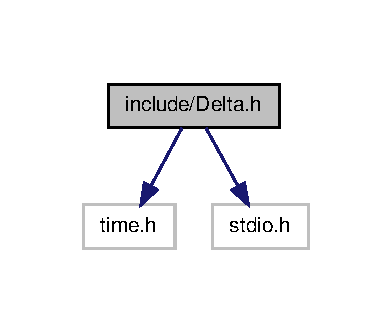
\includegraphics[width=188pt]{_delta_8h__incl}
\end{center}
\end{figure}
Dieser Graph zeigt, welche Datei direkt oder indirekt diese Datei enthält:\nopagebreak
\begin{figure}[H]
\begin{center}
\leavevmode
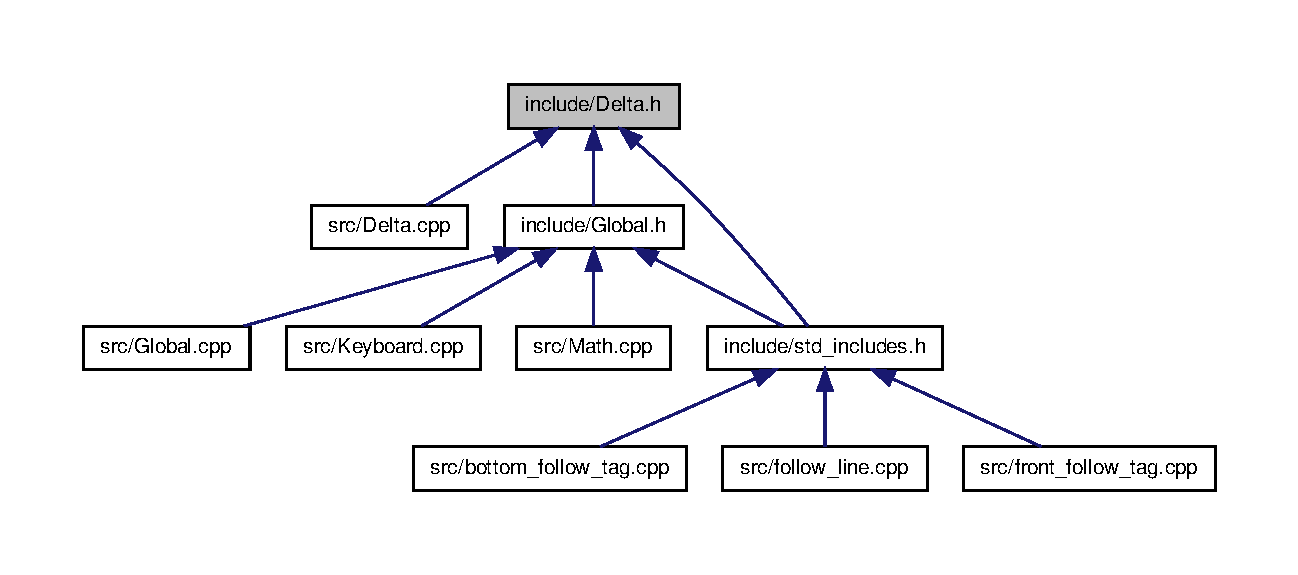
\includegraphics[width=162pt]{_delta_8h__dep__incl}
\end{center}
\end{figure}
\subsection*{Klassen}
\begin{DoxyCompactItemize}
\item 
class \hyperlink{class_delta}{Delta}
\begin{DoxyCompactList}\small\item\em Klasse, zur Berechnung der Geschwindigkeit (wird nicht mehr verwendet) \end{DoxyCompactList}\end{DoxyCompactItemize}


\subsection{Ausführliche Beschreibung}
Klasse, zur Berechnung der Geschwindigkeit (wird nicht mehr verwendet) 

Definiert in Datei \hyperlink{_delta_8h_source}{Delta.h}.


\hypertarget{_global_8h}{
\section{include/Global.h-\/Dateireferenz}
\label{_global_8h}\index{include/Global.h@{include/Global.h}}
}


Singleton: enthält alle Globalen Variablen.  


{\ttfamily \#include \char`\"{}std\_\-includes.h\char`\"{}}\par
Include-\/Abhängigkeitsdiagramm für Global.h:\nopagebreak
\begin{figure}[H]
\begin{center}
\leavevmode
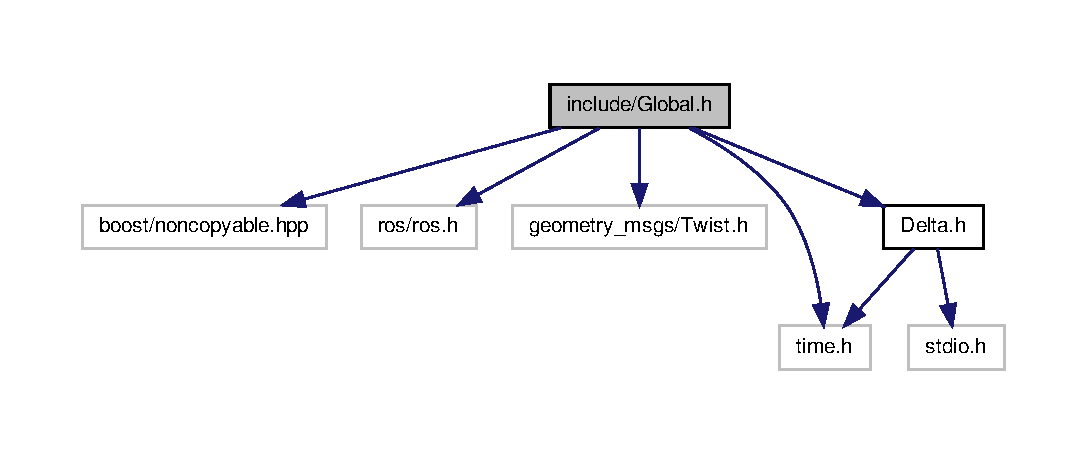
\includegraphics[width=400pt]{_global_8h__incl}
\end{center}
\end{figure}
Dieser Graph zeigt, welche Datei direkt oder indirekt diese Datei enthält:\nopagebreak
\begin{figure}[H]
\begin{center}
\leavevmode
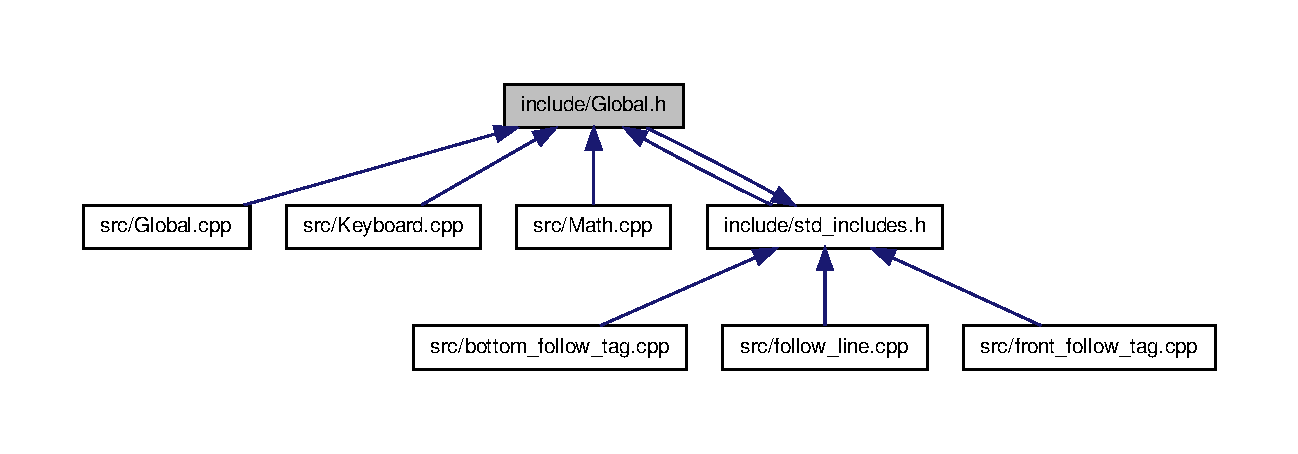
\includegraphics[width=400pt]{_global_8h__dep__incl}
\end{center}
\end{figure}
\subsection*{Klassen}
\begin{DoxyCompactItemize}
\item 
class \hyperlink{class_cglobal}{Cglobal}
\begin{DoxyCompactList}\small\item\em Klasse, die in Form eines Singletons alle globalen Variablen enthält. \end{DoxyCompactList}\end{DoxyCompactItemize}


\subsection{Ausführliche Beschreibung}
Singleton: enthält alle Globalen Variablen. 
\hypertarget{_keyboard_8h}{
\section{include/Keyboard.h-\/Dateireferenz}
\label{_keyboard_8h}\index{include/Keyboard.h@{include/Keyboard.h}}
}


enthält \hyperlink{namespace_keyboard_abfb3168172d115a6516147c6d42f58db}{Keyboard::control()} zum steuern der Drone mit der Tastatur  


Dieser Graph zeigt, welche Datei direkt oder indirekt diese Datei enthält:\nopagebreak
\begin{figure}[H]
\begin{center}
\leavevmode
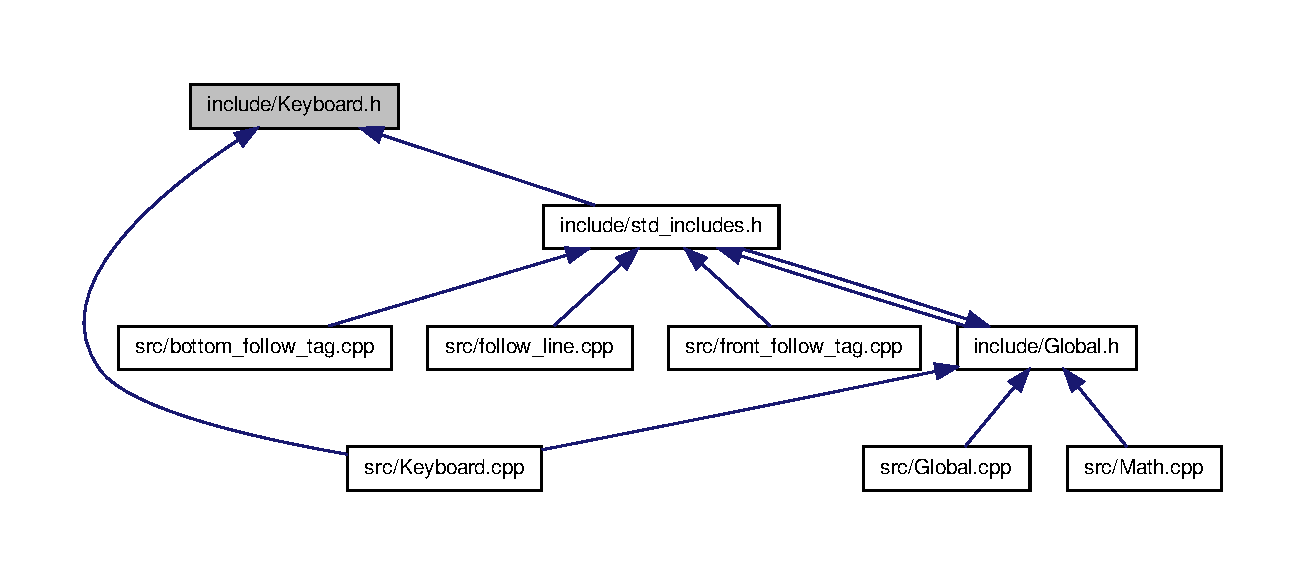
\includegraphics[width=400pt]{_keyboard_8h__dep__incl}
\end{center}
\end{figure}
\subsection*{Namensbereiche}
\begin{DoxyCompactItemize}
\item 
namespace \hyperlink{namespace_keyboard}{Keyboard}


\begin{DoxyCompactList}\small\item\em enthält \hyperlink{namespace_keyboard_abfb3168172d115a6516147c6d42f58db}{Keyboard::control()} zum steuern der Drone mit der Tastatur \end{DoxyCompactList}

\end{DoxyCompactItemize}
\subsection*{Funktionen}
\begin{DoxyCompactItemize}
\item 
void \hyperlink{namespace_keyboard_abfb3168172d115a6516147c6d42f58db}{Keyboard::control} ()
\begin{DoxyCompactList}\small\item\em zum Steuern der Drone mit der Tastatur \end{DoxyCompactList}\item 
int \hyperlink{namespace_keyboard_a8c142c603571175e17a83a9b99d00d63}{Keyboard::kbhit} ()
\begin{DoxyCompactList}\small\item\em gibt zurück, ob eine Taste gedrückt wurde \end{DoxyCompactList}\item 
int \hyperlink{namespace_keyboard_a433fc58fb356fe62305e8419dd7b33d6}{Keyboard::getch} ()
\begin{DoxyCompactList}\small\item\em gibt zurück, welche Taste gedrückt wurde \end{DoxyCompactList}\item 
void \hyperlink{namespace_keyboard_a6cc4fc3f7daf5630d0570f9d9d21d19c}{Keyboard::set\_\-conio\_\-terminal\_\-mode} ()
\item 
void \hyperlink{namespace_keyboard_aef945e5d33422ac6abbb326b5203eb5b}{Keyboard::reset\_\-terminal\_\-mode} ()
\end{DoxyCompactItemize}


\subsection{Ausführliche Beschreibung}
enthält \hyperlink{namespace_keyboard_abfb3168172d115a6516147c6d42f58db}{Keyboard::control()} zum steuern der Drone mit der Tastatur 
\hypertarget{_math_8h}{
\section{include/Math.h-\/Dateireferenz}
\label{_math_8h}\index{include/Math.h@{include/Math.h}}
}
{\ttfamily \#include \char`\"{}ar\_\-recog/Tag.h\char`\"{}}\par
{\ttfamily \#include \char`\"{}ardrone\_\-brown/Navdata.h\char`\"{}}\par
Include-\/Abhängigkeitsdiagramm für Math.h:\nopagebreak
\begin{figure}[H]
\begin{center}
\leavevmode
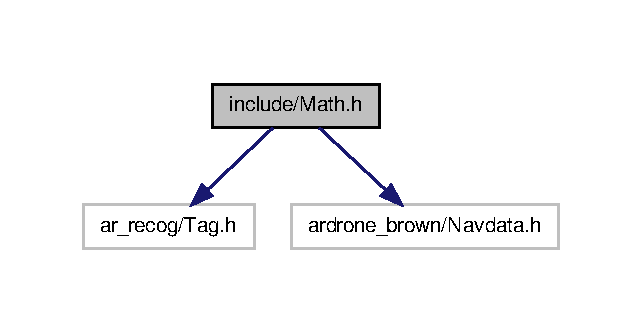
\includegraphics[width=308pt]{_math_8h__incl}
\end{center}
\end{figure}
Dieser Graph zeigt, welche Datei direkt oder indirekt diese Datei enthält:\nopagebreak
\begin{figure}[H]
\begin{center}
\leavevmode
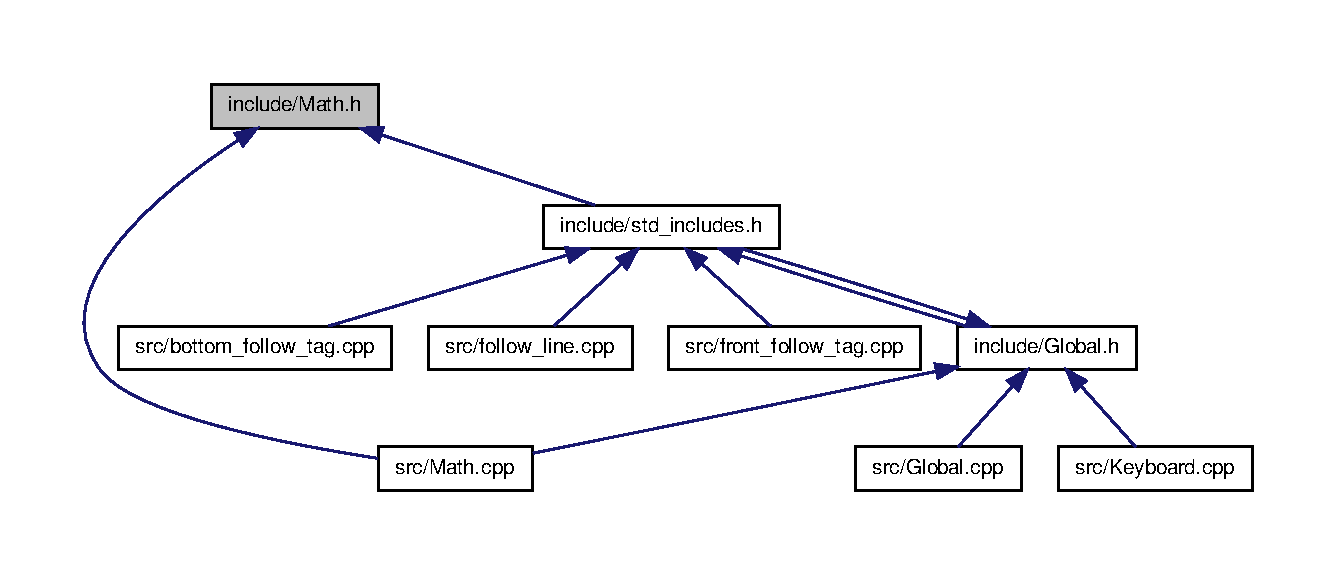
\includegraphics[width=400pt]{_math_8h__dep__incl}
\end{center}
\end{figure}
\subsection*{Namensbereiche}
\begin{DoxyCompactItemize}
\item 
namespace \hyperlink{namespace_math}{Math}
\end{DoxyCompactItemize}
\subsection*{Funktionen}
\begin{DoxyCompactItemize}
\item 
void \hyperlink{namespace_math_a25b9284eb485b732c952786b63343aaa}{Math::pixelDiffBottom} (float \&x, float \&y)
\begin{DoxyCompactList}\small\item\em Berechnung der Anzahl der Pixel für die Frontkamera, um die das Tag aufgrund der Rotation verschoben wurde. \end{DoxyCompactList}\item 
void \hyperlink{namespace_math_a3fbe7036db847d74ed5f2c21635d02d9}{Math::pixelDiffFront} (float \&x, float \&y)
\item 
void \hyperlink{namespace_math_ab4c584467f0cc5d8af22a69482630866}{Math::centerBottom} (const ar\_\-recog::Tag \&tag, float \&cx, float \&cy)
\begin{DoxyCompactList}\small\item\em Berechnung aus den Eckpunkten wo sich das Tag bezüglich des Bildes befindet. \end{DoxyCompactList}\item 
void \hyperlink{namespace_math_a43f025fac1ade5dbf88f7c393ca85644}{Math::centerFront} (const ar\_\-recog::Tag \&tag, float \&cx, float \&cy)
\item 
void \hyperlink{namespace_math_ad3b65f0aedda56076f681f2b987d0e5c}{Math::navdataUpdate} (const ardrone\_\-brown::Navdata::ConstPtr \&navdata)
\begin{DoxyCompactList}\small\item\em subscriber handler für die Nachricht /ardrone/navdata \end{DoxyCompactList}\end{DoxyCompactItemize}

\hypertarget{std__includes_8h}{
\section{include/std\_\-includes.h-\/Dateireferenz}
\label{std__includes_8h}\index{include/std\_\-includes.h@{include/std\_\-includes.h}}
}


included die Header, die standartmäßig benötigt werden  


{\ttfamily \#include $<$time.h$>$}\par
{\ttfamily \#include $<$stdio.h$>$}\par
{\ttfamily \#include $<$iostream$>$}\par
{\ttfamily \#include $<$sstream$>$}\par
{\ttfamily \#include $<$sys/time.h$>$}\par
{\ttfamily \#include $<$fstream$>$}\par
{\ttfamily \#include \char`\"{}ros/ros.h\char`\"{}}\par
{\ttfamily \#include \char`\"{}geometry\_\-msgs/Twist.h\char`\"{}}\par
{\ttfamily \#include \char`\"{}std\_\-msgs/Empty.h\char`\"{}}\par
{\ttfamily \#include \char`\"{}std\_\-msgs/String.h\char`\"{}}\par
{\ttfamily \#include \char`\"{}ar\_\-recog/Tags.h\char`\"{}}\par
{\ttfamily \#include \char`\"{}ar\_\-recog/Tag.h\char`\"{}}\par
{\ttfamily \#include \char`\"{}ardrone\_\-brown/Navdata.h\char`\"{}}\par
{\ttfamily \#include \char`\"{}Math.h\char`\"{}}\par
{\ttfamily \#include \char`\"{}Global.h\char`\"{}}\par
{\ttfamily \#include \char`\"{}Keyboard.h\char`\"{}}\par
Include-\/Abhängigkeitsdiagramm für std\_\-includes.h:\nopagebreak
\begin{figure}[H]
\begin{center}
\leavevmode
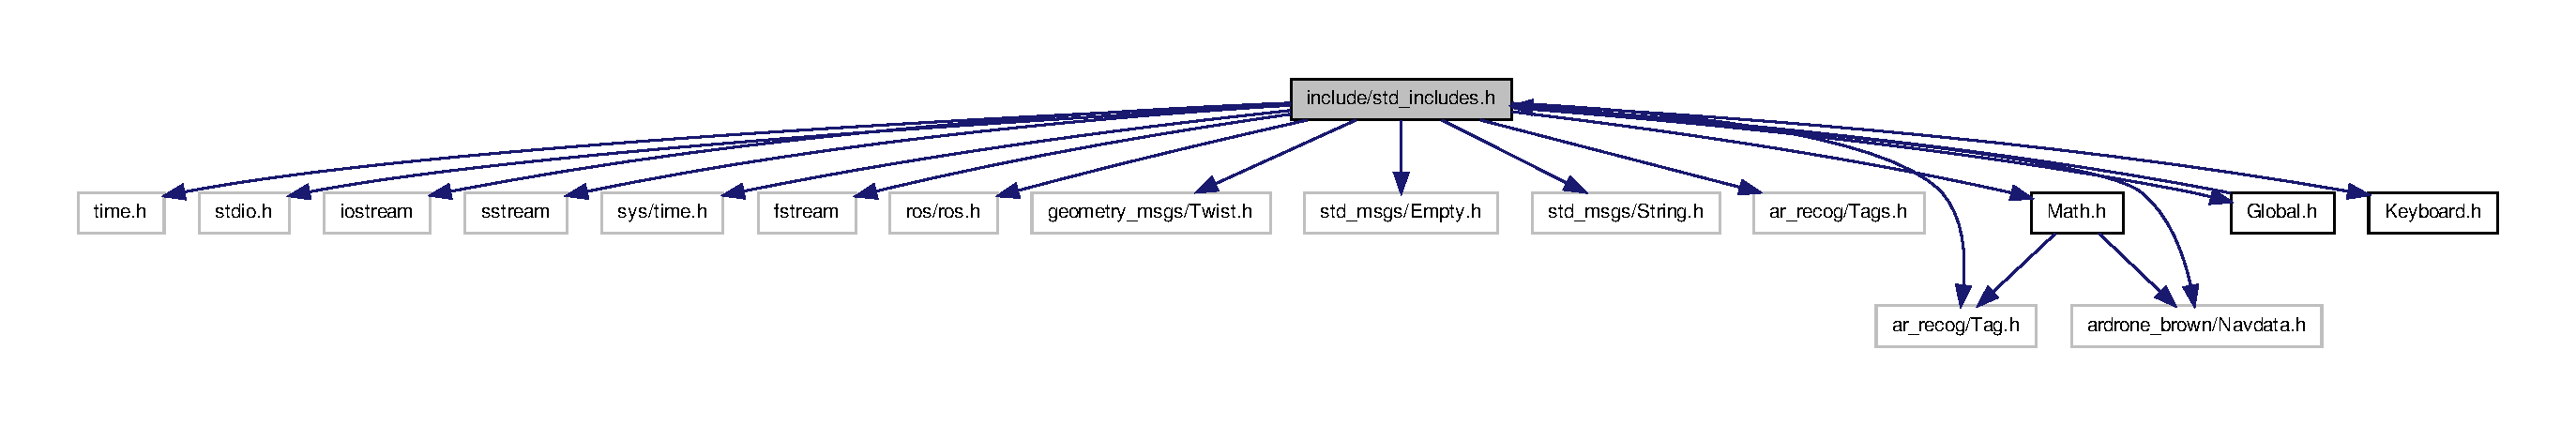
\includegraphics[width=400pt]{std__includes_8h__incl}
\end{center}
\end{figure}
Dieser Graph zeigt, welche Datei direkt oder indirekt diese Datei enthält:\nopagebreak
\begin{figure}[H]
\begin{center}
\leavevmode
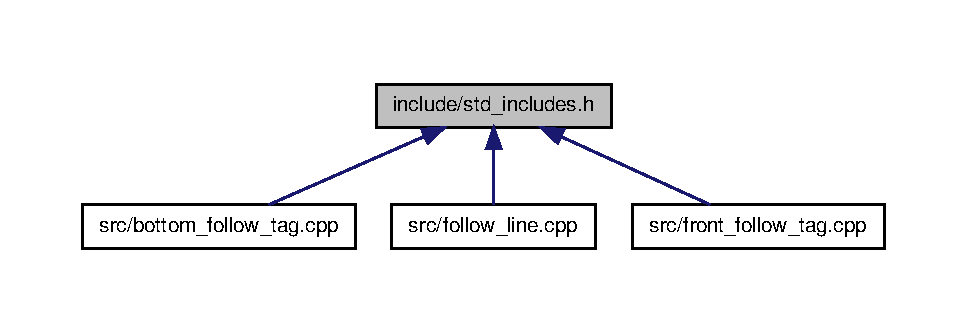
\includegraphics[width=400pt]{std__includes_8h__dep__incl}
\end{center}
\end{figure}


\subsection{Ausführliche Beschreibung}
included die Header, die standartmäßig benötigt werden 
\hypertarget{mainpage_8dox}{
\section{mainpage.dox-\/Dateireferenz}
\label{mainpage_8dox}\index{mainpage.dox@{mainpage.dox}}
}

\hypertarget{bottom__follow__tag_8cpp}{
\section{src/bottom\_\-follow\_\-tag.cpp-\/Dateireferenz}
\label{bottom__follow__tag_8cpp}\index{src/bottom\_\-follow\_\-tag.cpp@{src/bottom\_\-follow\_\-tag.cpp}}
}


Applikation zur Tagvervolgung mit der unteren Kamera.  


{\ttfamily \#include \char`\"{}std\_\-includes.h\char`\"{}}\par
\subsection*{Funktionen}
\begin{DoxyCompactItemize}
\item 
void \hyperlink{bottom__follow__tag_8cpp_a2379f8efc865258905edbf90e8678f69}{handleTag} (const ar\_\-recog::Tags::ConstPtr \&msg)
\begin{DoxyCompactList}\small\item\em handler für die Nachricht tags: hier werden die Bewegungsdaten gesetzt und gepublished \end{DoxyCompactList}\item 
int \hyperlink{bottom__follow__tag_8cpp_a3c04138a5bfe5d72780bb7e82a18e627}{main} (int argc, char $\ast$$\ast$argv)
\end{DoxyCompactItemize}


\subsection{Ausführliche Beschreibung}
Applikation zur Tagvervolgung mit der unteren Kamera. Die Applikation published eine Message vom Typ cmd\_\-vel(Twist-\/Objekt) zum steuern der Drone immer dann,\par
 wenn eine neue Message vom Typ tags von der Applikation ar\_\-recog gesendet wurde. Dies geschieht etwa 18 mal pro Sekunde. \par
\par
 Wurde ein Tag erkannt, soll die Drone darauf zu fliegen, sodass das Tag in den Mittelpunkt des Bildes kommt. \par
 Dabei fliegt die Drone bei einer Höhe von etwa 1,3m über dem Tag.\par
 Wurde kein Tag erkannt, fliegt die Drone drei Sekunden in die Richtung, in der sie das Tag zuletzt gesehen hat.\par
 Hat die Drone das Tag nach 3 Sekunden noch nicht wiedergefunden, fliegt sie auf der Stelle.\par
 \par
 Die Regelung erfolgt in \hyperlink{namespace_math_a688eccf4d1e0776ee10e6293254e2e13}{Math::bottom\_\-regulation()} mit Hilfe eines PD-\/Reglers.\par
 Sind über eine halbe Sekunde lang keine neuen Navigationsdaten(Message ardrone/navdata) von der Drone angekommen(passiert teilweise bei gestörter WLAN-\/Verbindung), \par
 bleibt die Drohne stehen. Sonst würde die Drone aufgrund der Regelung mit den alten Geschwindigkeitswerten nicht das gewünschte Verhalten zeigen. 

Definiert in Datei \hyperlink{bottom__follow__tag_8cpp_source}{bottom\_\-follow\_\-tag.cpp}.



\subsection{Dokumentation der Funktionen}
\hypertarget{bottom__follow__tag_8cpp_a2379f8efc865258905edbf90e8678f69}{
\index{bottom\_\-follow\_\-tag.cpp@{bottom\_\-follow\_\-tag.cpp}!handleTag@{handleTag}}
\index{handleTag@{handleTag}!bottom_follow_tag.cpp@{bottom\_\-follow\_\-tag.cpp}}
\subsubsection[{handleTag}]{\setlength{\rightskip}{0pt plus 5cm}void handleTag (
\begin{DoxyParamCaption}
\item[{const ar\_\-recog::Tags::ConstPtr \&}]{msg}
\end{DoxyParamCaption}
)}}
\label{bottom__follow__tag_8cpp_a2379f8efc865258905edbf90e8678f69}


handler für die Nachricht tags: hier werden die Bewegungsdaten gesetzt und gepublished 



Definiert in Zeile 27 der Datei bottom\_\-follow\_\-tag.cpp.

\hypertarget{bottom__follow__tag_8cpp_a3c04138a5bfe5d72780bb7e82a18e627}{
\index{bottom\_\-follow\_\-tag.cpp@{bottom\_\-follow\_\-tag.cpp}!main@{main}}
\index{main@{main}!bottom_follow_tag.cpp@{bottom\_\-follow\_\-tag.cpp}}
\subsubsection[{main}]{\setlength{\rightskip}{0pt plus 5cm}int main (
\begin{DoxyParamCaption}
\item[{int}]{argc, }
\item[{char $\ast$$\ast$}]{argv}
\end{DoxyParamCaption}
)}}
\label{bottom__follow__tag_8cpp_a3c04138a5bfe5d72780bb7e82a18e627}


Definiert in Zeile 115 der Datei bottom\_\-follow\_\-tag.cpp.


\hypertarget{_delta_8cpp}{
\section{src/Delta.cpp-\/Dateireferenz}
\label{_delta_8cpp}\index{src/Delta.cpp@{src/Delta.cpp}}
}
{\ttfamily \#include \char`\"{}Delta.h\char`\"{}}\par
{\ttfamily \#include $<$time.h$>$}\par
{\ttfamily \#include $<$stdio.h$>$}\par

\hypertarget{follow__line_8cpp}{
\section{src/follow\_\-line.cpp-\/Dateireferenz}
\label{follow__line_8cpp}\index{src/follow\_\-line.cpp@{src/follow\_\-line.cpp}}
}


Applikation zur Linienverfolgung mit der unteren Kamera.  


{\ttfamily \#include \char`\"{}std\_\-includes.h\char`\"{}}\par
{\ttfamily \#include \char`\"{}ardrone\_\-swp/LinePos.h\char`\"{}}\par
Include-\/Abhängigkeitsdiagramm für follow\_\-line.cpp:\nopagebreak
\begin{figure}[H]
\begin{center}
\leavevmode
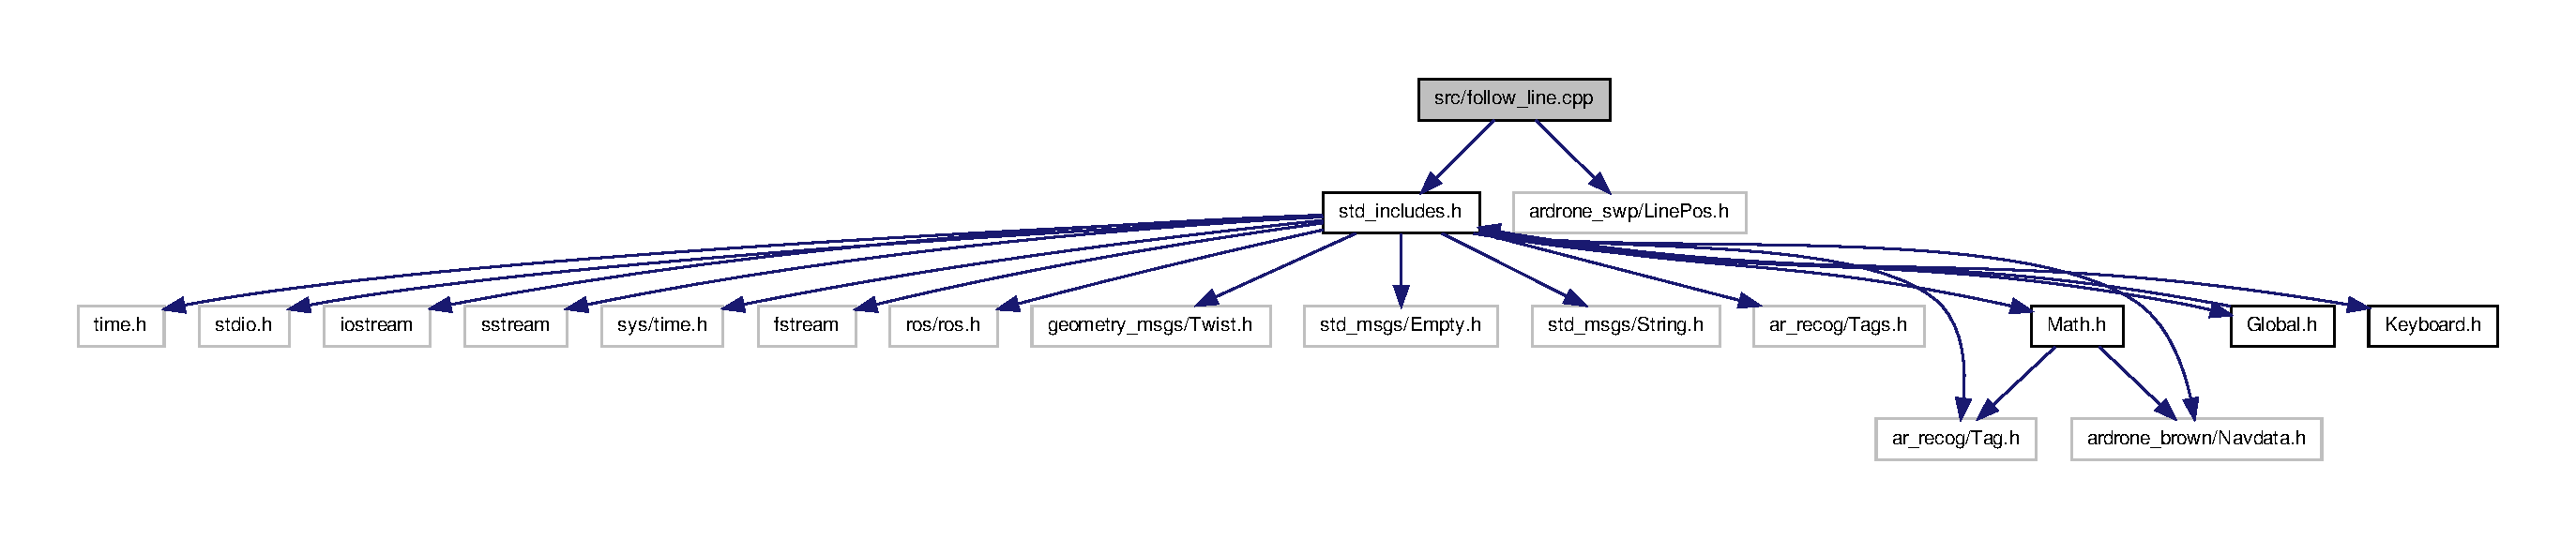
\includegraphics[width=400pt]{follow__line_8cpp__incl}
\end{center}
\end{figure}
\subsection*{Funktionen}
\begin{DoxyCompactItemize}
\item 
void \hyperlink{follow__line_8cpp_a35a859d19785b808898bf535d4997d2f}{handleLine} (const ardrone\_\-swp::LinePos::ConstPtr \&msg)
\item 
int \hyperlink{follow__line_8cpp_a3c04138a5bfe5d72780bb7e82a18e627}{main} (int argc, char $\ast$$\ast$argv)
\end{DoxyCompactItemize}


\subsection{Ausführliche Beschreibung}
Applikation zur Linienverfolgung mit der unteren Kamera. 

\subsection{Dokumentation der Funktionen}
\hypertarget{follow__line_8cpp_a35a859d19785b808898bf535d4997d2f}{
\index{follow\_\-line.cpp@{follow\_\-line.cpp}!handleLine@{handleLine}}
\index{handleLine@{handleLine}!follow_line.cpp@{follow\_\-line.cpp}}
\subsubsection[{handleLine}]{\setlength{\rightskip}{0pt plus 5cm}void handleLine (
\begin{DoxyParamCaption}
\item[{const ardrone\_\-swp::LinePos::ConstPtr \&}]{msg}
\end{DoxyParamCaption}
)}}
\label{follow__line_8cpp_a35a859d19785b808898bf535d4997d2f}


Hier ist ein Graph der zeigt, was diese Funktion aufruft:\nopagebreak
\begin{figure}[H]
\begin{center}
\leavevmode
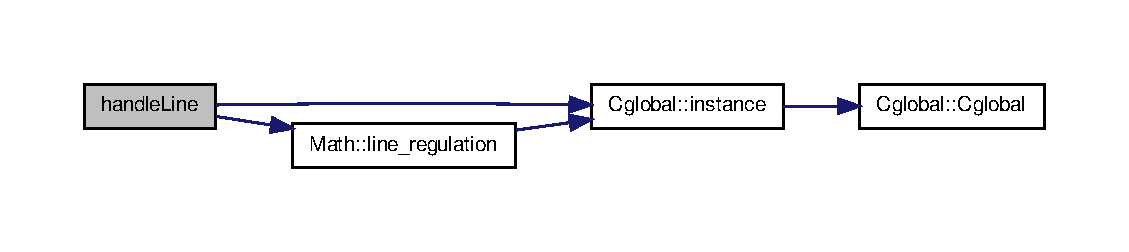
\includegraphics[width=400pt]{follow__line_8cpp_a35a859d19785b808898bf535d4997d2f_cgraph}
\end{center}
\end{figure}




Hier ist ein Graph der zeigt, wo diese Funktion aufgerufen wird:\nopagebreak
\begin{figure}[H]
\begin{center}
\leavevmode
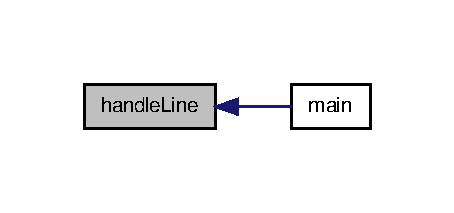
\includegraphics[width=218pt]{follow__line_8cpp_a35a859d19785b808898bf535d4997d2f_icgraph}
\end{center}
\end{figure}


\hypertarget{follow__line_8cpp_a3c04138a5bfe5d72780bb7e82a18e627}{
\index{follow\_\-line.cpp@{follow\_\-line.cpp}!main@{main}}
\index{main@{main}!follow_line.cpp@{follow\_\-line.cpp}}
\subsubsection[{main}]{\setlength{\rightskip}{0pt plus 5cm}int main (
\begin{DoxyParamCaption}
\item[{int}]{argc, }
\item[{char $\ast$$\ast$}]{argv}
\end{DoxyParamCaption}
)}}
\label{follow__line_8cpp_a3c04138a5bfe5d72780bb7e82a18e627}


Hier ist ein Graph der zeigt, was diese Funktion aufruft:\nopagebreak
\begin{figure}[H]
\begin{center}
\leavevmode
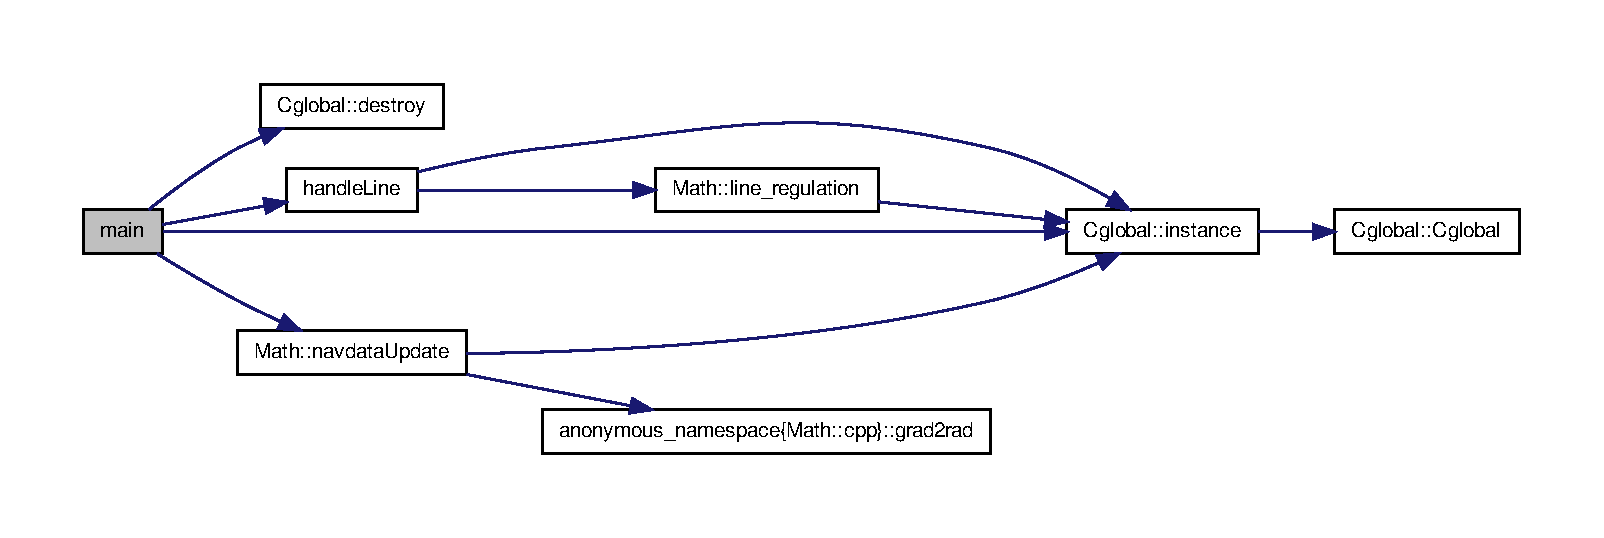
\includegraphics[width=400pt]{follow__line_8cpp_a3c04138a5bfe5d72780bb7e82a18e627_cgraph}
\end{center}
\end{figure}



\hypertarget{front__follow__tag_8cpp}{
\section{src/front\_\-follow\_\-tag.cpp-\/Dateireferenz}
\label{front__follow__tag_8cpp}\index{src/front\_\-follow\_\-tag.cpp@{src/front\_\-follow\_\-tag.cpp}}
}


Applikation zur Tagvervolgung mit der vorderen Kamera.  


{\ttfamily \#include \char`\"{}std\_\-includes.h\char`\"{}}\par
Include-\/Abhängigkeitsdiagramm für front\_\-follow\_\-tag.cpp:\nopagebreak
\begin{figure}[H]
\begin{center}
\leavevmode
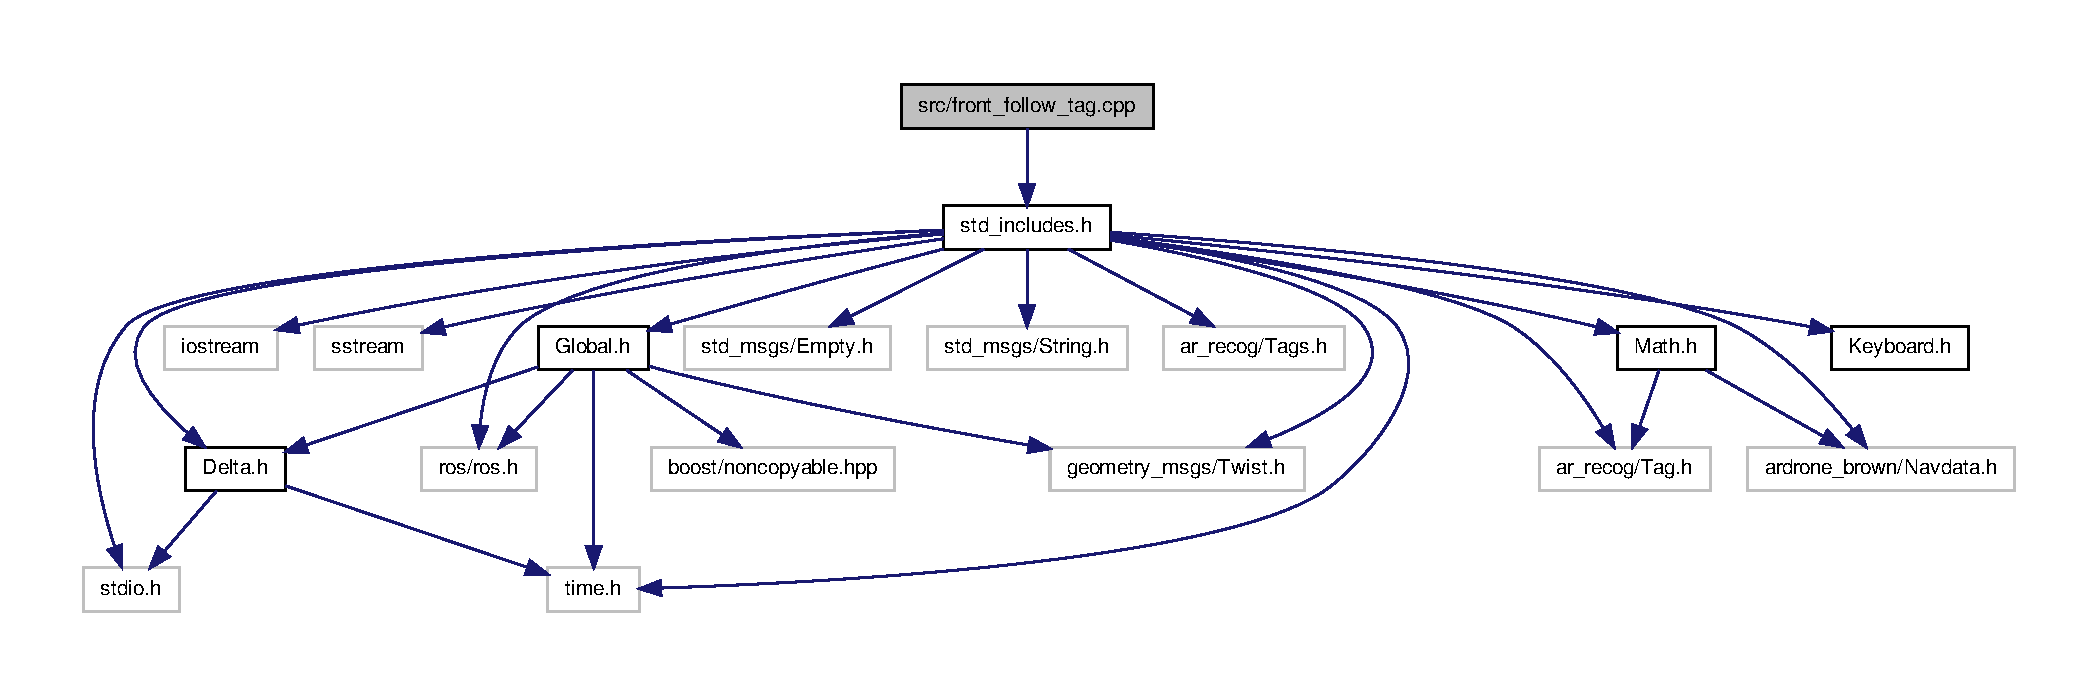
\includegraphics[width=400pt]{front__follow__tag_8cpp__incl}
\end{center}
\end{figure}
\subsection*{Funktionen}
\begin{DoxyCompactItemize}
\item 
void \hyperlink{front__follow__tag_8cpp_a2379f8efc865258905edbf90e8678f69}{handleTag} (const ar\_\-recog::Tags::ConstPtr \&msg)
\begin{DoxyCompactList}\small\item\em handler für die Nachricht tags hier werden die Bewegungsdaten gesetzt und gepublished \end{DoxyCompactList}\item 
int \hyperlink{front__follow__tag_8cpp_a3c04138a5bfe5d72780bb7e82a18e627}{main} (int argc, char $\ast$$\ast$argv)
\end{DoxyCompactItemize}


\subsection{Ausführliche Beschreibung}
Applikation zur Tagvervolgung mit der vorderen Kamera. TODO : Ausführliche Beschreibung 

\subsection{Dokumentation der Funktionen}
\hypertarget{front__follow__tag_8cpp_a2379f8efc865258905edbf90e8678f69}{
\index{front\_\-follow\_\-tag.cpp@{front\_\-follow\_\-tag.cpp}!handleTag@{handleTag}}
\index{handleTag@{handleTag}!front_follow_tag.cpp@{front\_\-follow\_\-tag.cpp}}
\subsubsection[{handleTag}]{\setlength{\rightskip}{0pt plus 5cm}void handleTag (
\begin{DoxyParamCaption}
\item[{const ar\_\-recog::Tags::ConstPtr \&}]{msg}
\end{DoxyParamCaption}
)}}
\label{front__follow__tag_8cpp_a2379f8efc865258905edbf90e8678f69}


handler für die Nachricht tags hier werden die Bewegungsdaten gesetzt und gepublished 

TODO : Ausführliche Beschreibung 

Hier ist ein Graph der zeigt, was diese Funktion aufruft:\nopagebreak
\begin{figure}[H]
\begin{center}
\leavevmode
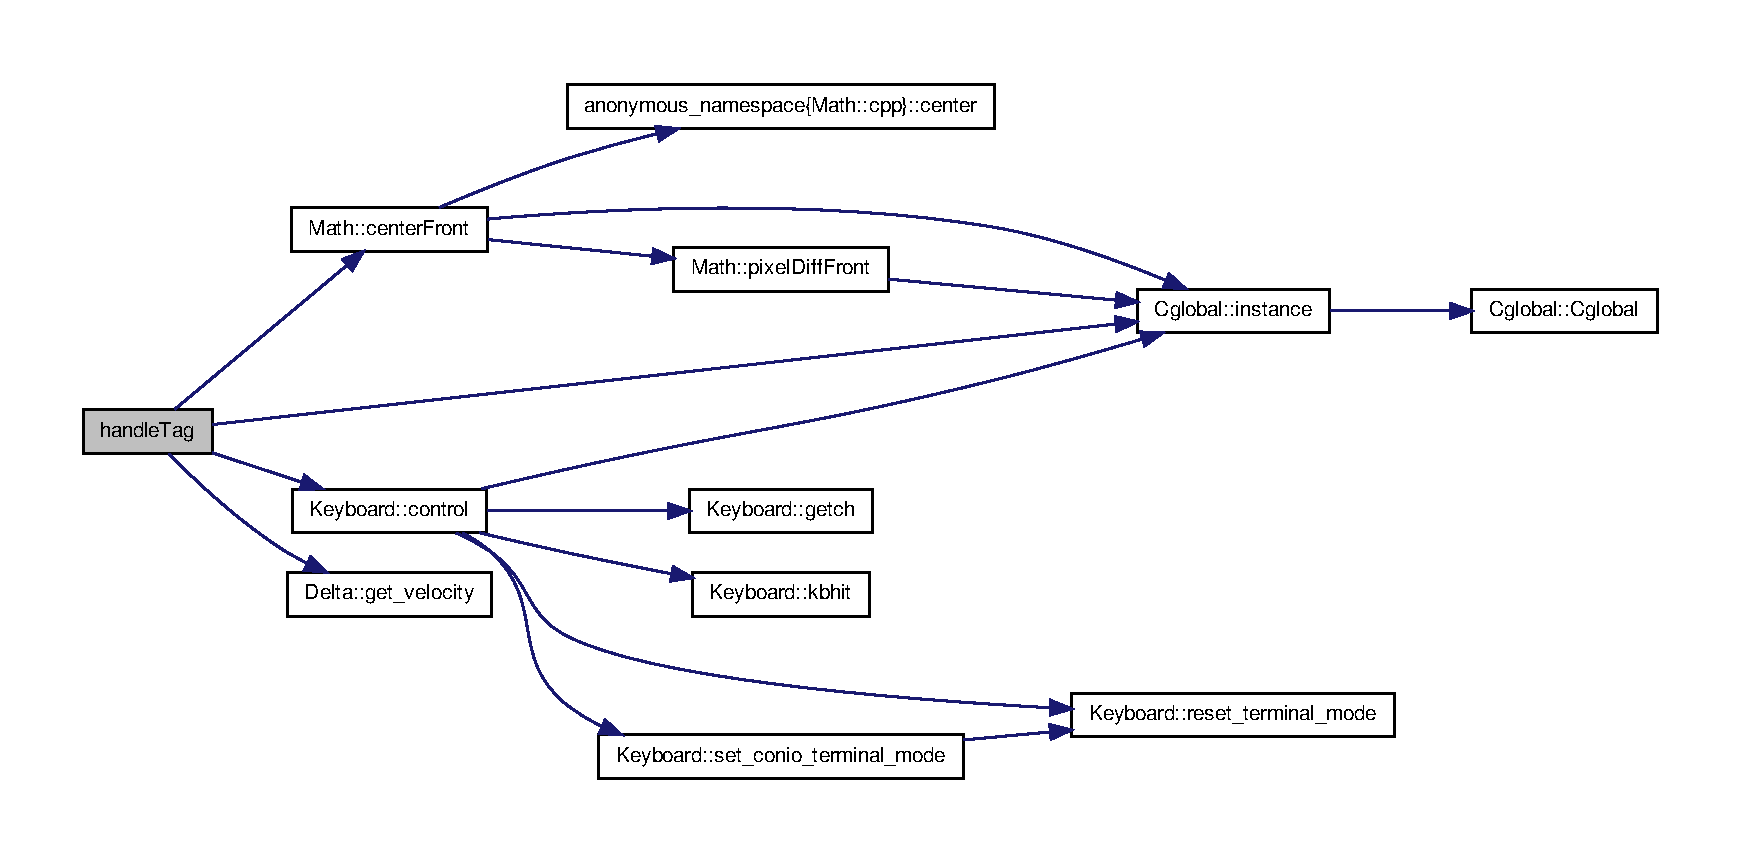
\includegraphics[width=400pt]{front__follow__tag_8cpp_a2379f8efc865258905edbf90e8678f69_cgraph}
\end{center}
\end{figure}


\hypertarget{front__follow__tag_8cpp_a3c04138a5bfe5d72780bb7e82a18e627}{
\index{front\_\-follow\_\-tag.cpp@{front\_\-follow\_\-tag.cpp}!main@{main}}
\index{main@{main}!front_follow_tag.cpp@{front\_\-follow\_\-tag.cpp}}
\subsubsection[{main}]{\setlength{\rightskip}{0pt plus 5cm}int main (
\begin{DoxyParamCaption}
\item[{int}]{argc, }
\item[{char $\ast$$\ast$}]{argv}
\end{DoxyParamCaption}
)}}
\label{front__follow__tag_8cpp_a3c04138a5bfe5d72780bb7e82a18e627}


Hier ist ein Graph der zeigt, was diese Funktion aufruft:\nopagebreak
\begin{figure}[H]
\begin{center}
\leavevmode
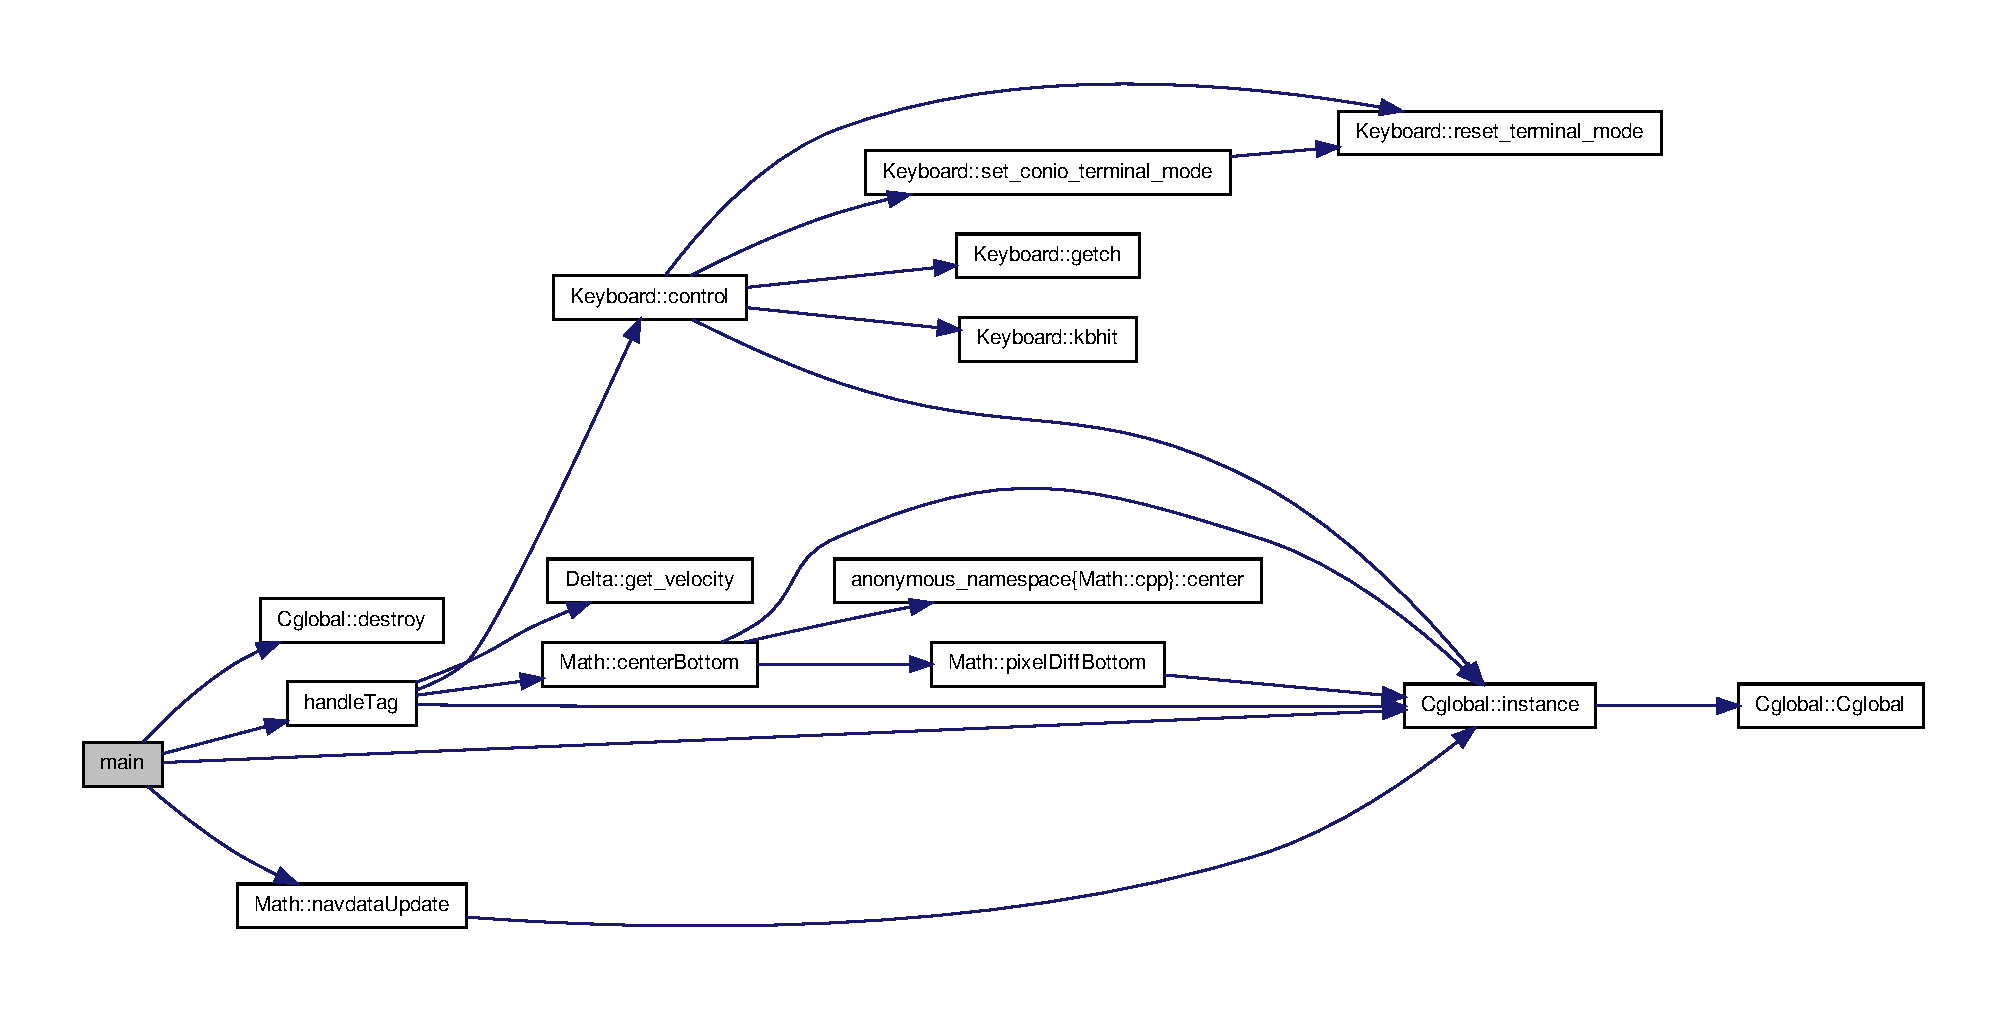
\includegraphics[width=400pt]{front__follow__tag_8cpp_a3c04138a5bfe5d72780bb7e82a18e627_cgraph}
\end{center}
\end{figure}



\hypertarget{_global_8cpp}{
\section{src/Global.cpp-\/Dateireferenz}
\label{_global_8cpp}\index{src/Global.cpp@{src/Global.cpp}}
}
{\ttfamily \#include \char`\"{}Global.h\char`\"{}}\par
{\ttfamily \#include $<$time.h$>$}\par

\hypertarget{_keyboard_8cpp}{
\section{src/Keyboard.cpp-\/Dateireferenz}
\label{_keyboard_8cpp}\index{src/Keyboard.cpp@{src/Keyboard.cpp}}
}
{\ttfamily \#include \char`\"{}Keyboard.h\char`\"{}}\par
{\ttfamily \#include \char`\"{}Global.h\char`\"{}}\par
{\ttfamily \#include $<$stdlib.h$>$}\par
{\ttfamily \#include $<$string.h$>$}\par
{\ttfamily \#include $<$sys/select.h$>$}\par
{\ttfamily \#include $<$termios.h$>$}\par
{\ttfamily \#include $<$sstream$>$}\par
Include-\/Abhängigkeitsdiagramm für Keyboard.cpp:\nopagebreak
\begin{figure}[H]
\begin{center}
\leavevmode
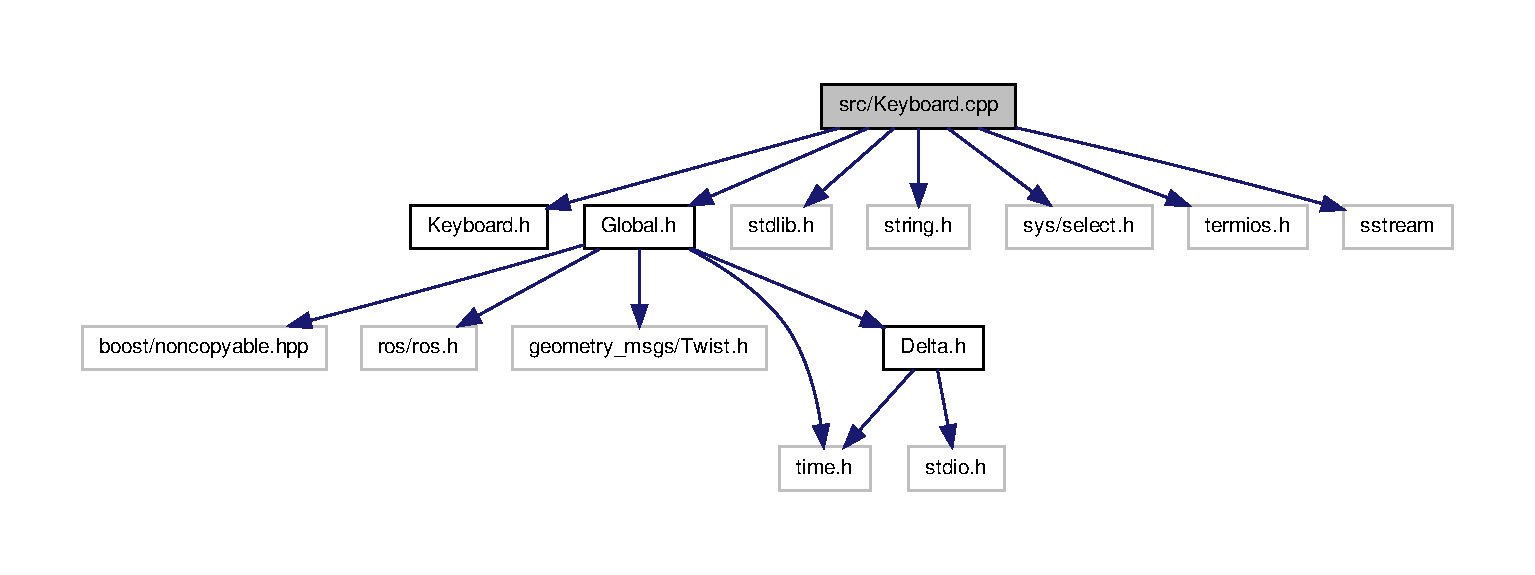
\includegraphics[width=400pt]{_keyboard_8cpp__incl}
\end{center}
\end{figure}
\subsection*{Namensbereiche}
\begin{DoxyCompactItemize}
\item 
namespace \hyperlink{namespace_keyboard}{Keyboard}
\end{DoxyCompactItemize}
\subsection*{Funktionen}
\begin{DoxyCompactItemize}
\item 
void \hyperlink{namespace_keyboard_abfb3168172d115a6516147c6d42f58db}{Keyboard::control} ()
\begin{DoxyCompactList}\small\item\em zum Steuern der Drone mit der Tastatur \end{DoxyCompactList}\item 
void \hyperlink{namespace_keyboard_aef945e5d33422ac6abbb326b5203eb5b}{Keyboard::reset\_\-terminal\_\-mode} ()
\item 
void \hyperlink{namespace_keyboard_a6cc4fc3f7daf5630d0570f9d9d21d19c}{Keyboard::set\_\-conio\_\-terminal\_\-mode} ()
\item 
int \hyperlink{namespace_keyboard_a8c142c603571175e17a83a9b99d00d63}{Keyboard::kbhit} ()
\item 
int \hyperlink{namespace_keyboard_a433fc58fb356fe62305e8419dd7b33d6}{Keyboard::getch} ()
\end{DoxyCompactItemize}
\subsection*{Variablen}
\begin{DoxyCompactItemize}
\item 
struct termios \hyperlink{namespace_keyboard_a8b623d5192e406c97c4e265dbe4c5f38}{Keyboard::orig\_\-termios}
\end{DoxyCompactItemize}

\hypertarget{_log_8cpp}{
\section{src/Log.cpp-\/Dateireferenz}
\label{_log_8cpp}\index{src/Log.cpp@{src/Log.cpp}}
}


Applikation zum Loggen der Navdata, Twist, Tags.  


{\ttfamily \#include \char`\"{}ardrone\_\-brown/Navdata.h\char`\"{}}\par
{\ttfamily \#include \char`\"{}ros/ros.h\char`\"{}}\par
{\ttfamily \#include \char`\"{}ar\_\-recog/Tags.h\char`\"{}}\par
{\ttfamily \#include \char`\"{}ar\_\-recog/Tag.h\char`\"{}}\par
{\ttfamily \#include \char`\"{}geometry\_\-msgs/Twist.h\char`\"{}}\par
{\ttfamily \#include $<$time.h$>$}\par
{\ttfamily \#include $<$stdio.h$>$}\par
{\ttfamily \#include $<$iostream$>$}\par
{\ttfamily \#include $<$sstream$>$}\par
{\ttfamily \#include $<$fstream$>$}\par
{\ttfamily \#include $<$sys/time.h$>$}\par
{\ttfamily \#include $<$boost/filesystem.hpp$>$}\par
\subsection*{Funktionen}
\begin{DoxyCompactItemize}
\item 
void \hyperlink{_log_8cpp_a2379f8efc865258905edbf90e8678f69}{handleTag} (const ar\_\-recog::Tags::ConstPtr \&msg)
\begin{DoxyCompactList}\small\item\em schreibt die Tag-\/Informationen in die entsprechende Datei \end{DoxyCompactList}\item 
void \hyperlink{_log_8cpp_a39bd57f05a0879f1d9df4e82bfbfa30e}{navdataUpdate} (const ardrone\_\-brown::Navdata::ConstPtr \&navdata)
\begin{DoxyCompactList}\small\item\em schreibt die Navdata-\/Informationen in die entsprechende Datei \end{DoxyCompactList}\item 
void \hyperlink{_log_8cpp_a2fa433d675a4836a65893acd6d27f0f5}{handleTwist} (const geometry\_\-msgs::TwistConstPtr \&msg)
\begin{DoxyCompactList}\small\item\em schreibt die Twist-\/Informationen in die entsprechende Datei \end{DoxyCompactList}\item 
int \hyperlink{_log_8cpp_a3c04138a5bfe5d72780bb7e82a18e627}{main} (int argc, char $\ast$$\ast$argv)
\end{DoxyCompactItemize}
\subsection*{Variablen}
\begin{DoxyCompactItemize}
\item 
ofstream \hyperlink{_log_8cpp_a23aa93e4ff6c46053ab418dc360e4f1a}{logNavdata}
\item 
ofstream \hyperlink{_log_8cpp_a3dac8915f5e71afcc09a40bae7c7d802}{logTags}
\item 
ofstream \hyperlink{_log_8cpp_a10bb79822b487dbc4db2b1b64a8ea80a}{logTwist}
\end{DoxyCompactItemize}


\subsection{Ausführliche Beschreibung}
Applikation zum Loggen der Navdata, Twist, Tags. Option, die beim Aufruf übergeben werden können:

n : Navdata loggen

t : Tags loggen

w : gesentete Twist-\/Objekte loggen

Beispielsaufruf: rosrun ardrone\_\-swp Log n w t

-\/$>$loggt Navtada, Tags und Twist-\/Objekte

wird in die Ornder: ardrone\_\-swp/Log/ mit den Unterorndern LogNavdata, LogTags, LogTwist geschrieben

Die Dateinahmen sind das aktuelle Datum 

Definiert in Datei \hyperlink{_log_8cpp_source}{Log.cpp}.



\subsection{Dokumentation der Funktionen}
\hypertarget{_log_8cpp_a2379f8efc865258905edbf90e8678f69}{
\index{Log.cpp@{Log.cpp}!handleTag@{handleTag}}
\index{handleTag@{handleTag}!Log.cpp@{Log.cpp}}
\subsubsection[{handleTag}]{\setlength{\rightskip}{0pt plus 5cm}void handleTag (
\begin{DoxyParamCaption}
\item[{const ar\_\-recog::Tags::ConstPtr \&}]{msg}
\end{DoxyParamCaption}
)}}
\label{_log_8cpp_a2379f8efc865258905edbf90e8678f69}


schreibt die Tag-\/Informationen in die entsprechende Datei 



Definiert in Zeile 48 der Datei Log.cpp.

\hypertarget{_log_8cpp_a2fa433d675a4836a65893acd6d27f0f5}{
\index{Log.cpp@{Log.cpp}!handleTwist@{handleTwist}}
\index{handleTwist@{handleTwist}!Log.cpp@{Log.cpp}}
\subsubsection[{handleTwist}]{\setlength{\rightskip}{0pt plus 5cm}void handleTwist (
\begin{DoxyParamCaption}
\item[{const geometry\_\-msgs::TwistConstPtr \&}]{msg}
\end{DoxyParamCaption}
)}}
\label{_log_8cpp_a2fa433d675a4836a65893acd6d27f0f5}


schreibt die Twist-\/Informationen in die entsprechende Datei 



Definiert in Zeile 101 der Datei Log.cpp.

\hypertarget{_log_8cpp_a3c04138a5bfe5d72780bb7e82a18e627}{
\index{Log.cpp@{Log.cpp}!main@{main}}
\index{main@{main}!Log.cpp@{Log.cpp}}
\subsubsection[{main}]{\setlength{\rightskip}{0pt plus 5cm}int main (
\begin{DoxyParamCaption}
\item[{int}]{argc, }
\item[{char $\ast$$\ast$}]{argv}
\end{DoxyParamCaption}
)}}
\label{_log_8cpp_a3c04138a5bfe5d72780bb7e82a18e627}


Definiert in Zeile 114 der Datei Log.cpp.

\hypertarget{_log_8cpp_a39bd57f05a0879f1d9df4e82bfbfa30e}{
\index{Log.cpp@{Log.cpp}!navdataUpdate@{navdataUpdate}}
\index{navdataUpdate@{navdataUpdate}!Log.cpp@{Log.cpp}}
\subsubsection[{navdataUpdate}]{\setlength{\rightskip}{0pt plus 5cm}void navdataUpdate (
\begin{DoxyParamCaption}
\item[{const ardrone\_\-brown::Navdata::ConstPtr \&}]{navdata}
\end{DoxyParamCaption}
)}}
\label{_log_8cpp_a39bd57f05a0879f1d9df4e82bfbfa30e}


schreibt die Navdata-\/Informationen in die entsprechende Datei 



Definiert in Zeile 83 der Datei Log.cpp.



\subsection{Variablen-\/Dokumentation}
\hypertarget{_log_8cpp_a23aa93e4ff6c46053ab418dc360e4f1a}{
\index{Log.cpp@{Log.cpp}!logNavdata@{logNavdata}}
\index{logNavdata@{logNavdata}!Log.cpp@{Log.cpp}}
\subsubsection[{logNavdata}]{\setlength{\rightskip}{0pt plus 5cm}ofstream {\bf logNavdata}}}
\label{_log_8cpp_a23aa93e4ff6c46053ab418dc360e4f1a}


Definiert in Zeile 41 der Datei Log.cpp.

\hypertarget{_log_8cpp_a3dac8915f5e71afcc09a40bae7c7d802}{
\index{Log.cpp@{Log.cpp}!logTags@{logTags}}
\index{logTags@{logTags}!Log.cpp@{Log.cpp}}
\subsubsection[{logTags}]{\setlength{\rightskip}{0pt plus 5cm}ofstream {\bf logTags}}}
\label{_log_8cpp_a3dac8915f5e71afcc09a40bae7c7d802}


Definiert in Zeile 42 der Datei Log.cpp.

\hypertarget{_log_8cpp_a10bb79822b487dbc4db2b1b64a8ea80a}{
\index{Log.cpp@{Log.cpp}!logTwist@{logTwist}}
\index{logTwist@{logTwist}!Log.cpp@{Log.cpp}}
\subsubsection[{logTwist}]{\setlength{\rightskip}{0pt plus 5cm}ofstream {\bf logTwist}}}
\label{_log_8cpp_a10bb79822b487dbc4db2b1b64a8ea80a}


Definiert in Zeile 43 der Datei Log.cpp.


\hypertarget{_math_8cpp}{
\section{src/Math.cpp-\/Dateireferenz}
\label{_math_8cpp}\index{src/Math.cpp@{src/Math.cpp}}
}
{\ttfamily \#include \char`\"{}Math.h\char`\"{}}\par
{\ttfamily \#include \char`\"{}Global.h\char`\"{}}\par
{\ttfamily \#include \char`\"{}ardrone\_\-brown/Navdata.h\char`\"{}}\par
Include-\/Abhängigkeitsdiagramm für Math.cpp:\nopagebreak
\begin{figure}[H]
\begin{center}
\leavevmode
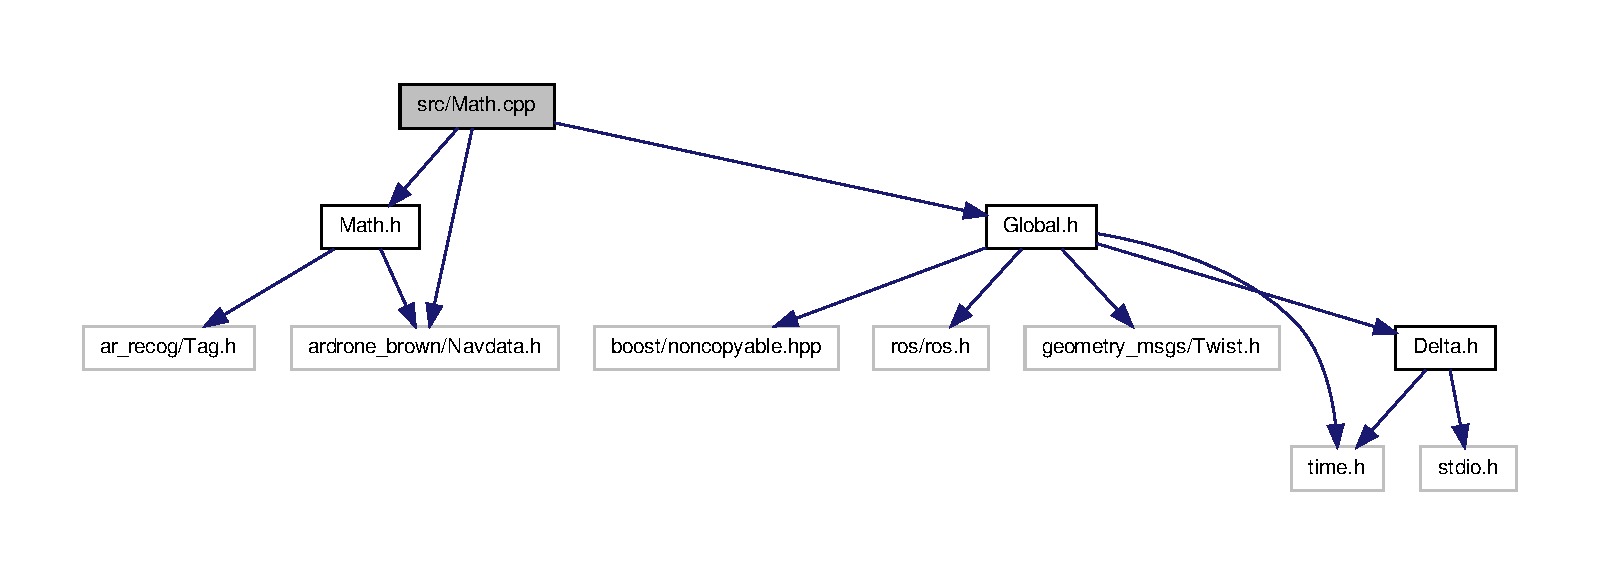
\includegraphics[width=400pt]{_math_8cpp__incl}
\end{center}
\end{figure}
\subsection*{Namensbereiche}
\begin{DoxyCompactItemize}
\item 
namespace \hyperlink{namespaceanonymous__namespace_02_math_8cpp_03}{anonymous\_\-namespace\{Math.cpp\}}
\item 
namespace \hyperlink{namespace_math}{Math}
\end{DoxyCompactItemize}
\subsection*{Funktionen}
\begin{DoxyCompactItemize}
\item 
void \hyperlink{namespaceanonymous__namespace_02_math_8cpp_03_af32b12f59241277b0b94ca38ca1d5a4b}{anonymous\_\-namespace\{Math.cpp\}::center} (const ar\_\-recog::Tag \&tag, float \&cx, float \&cy, float dx, float dy, float width, float height)
\item 
void \hyperlink{namespace_math_a25b9284eb485b732c952786b63343aaa}{Math::pixelDiffBottom} (float \&x, float \&y)
\begin{DoxyCompactList}\small\item\em Berechnung der Anzahl der Pixel für die Frontkamera, um die das Tag aufgrund der Rotation verschoben wurde. \end{DoxyCompactList}\item 
void \hyperlink{namespace_math_a3fbe7036db847d74ed5f2c21635d02d9}{Math::pixelDiffFront} (float \&x, float \&y)
\item 
void \hyperlink{namespace_math_ab4c584467f0cc5d8af22a69482630866}{Math::centerBottom} (const ar\_\-recog::Tag \&tag, float \&cx, float \&cy)
\begin{DoxyCompactList}\small\item\em Berechnung aus den Eckpunkten wo sich das Tag bezüglich des Bildes befindet. \end{DoxyCompactList}\item 
void \hyperlink{namespace_math_a43f025fac1ade5dbf88f7c393ca85644}{Math::centerFront} (const ar\_\-recog::Tag \&tag, float \&cx, float \&cy)
\item 
void \hyperlink{namespace_math_ad3b65f0aedda56076f681f2b987d0e5c}{Math::navdataUpdate} (const ardrone\_\-brown::Navdata::ConstPtr \&navdata)
\begin{DoxyCompactList}\small\item\em subscriber handler für die Nachricht /ardrone/navdata \end{DoxyCompactList}\end{DoxyCompactItemize}

\printindex
\end{document}
